\documentclass[12pt]{beamer}
\usepackage[utf8]{inputenc}
\usepackage[spanish]{babel}
\usepackage{color}
\usepackage{hyperref}
\usepackage{amsmath}
\usepackage{amsthm}
\usepackage{multicol}
\usepackage{graphicx}
\usepackage{tikz}
\usepackage[autostyle,spanish=mexican]{csquotes}
%\usepackage[sfdefault]{roboto}  %% Option 'sfdefault' only if the base font of the document is to be sans serif
\renewcommand{\arraystretch}{1.5}
\renewcommand{\rmdefault}{cmr}% cmr = Computer Modern Roman
\usefonttheme[onlymath]{serif}

\newcommand{\python}{\texttt{python}}
\newcommand{\textoazul}[1]{\textcolor{blue}{#1}}
\newcommand{\azulfuerte}[1]{\textcolor{blue}{\textbf{#1}}}
\newcounter{saveenumi}
\newcommand{\seti}{\setcounter{saveenumi}{\value{enumi}}}
\newcommand{\conti}{\setcounter{enumi}{\value{saveenumi}}}

\linespread{1.5}
\beamertemplatenavigationsymbolsempty
\usefonttheme{professionalfonts}
\usefonttheme{serif}
\DeclareGraphicsExtensions{.pdf,.png,.jpg}
\renewcommand {\arraystretch}{1.25}
\mode<presentation>
{
  \usetheme{Warsaw}
  \setbeamertemplate{headline}{}
  %\useoutertheme{infolines}
  \useoutertheme{default}
  \setbeamercovered{invisible}
  % or whatever (possibly just delete it)
  \setbeamertemplate{section in toc}[sections numbered]
  \setbeamertemplate{subsection in toc}[subsections numbered]
  \setbeamertemplate{subsection in toc}{\leavevmode\leftskip=3.2em\rlap{\hskip-2em\inserttocsectionnumber.\inserttocsubsectionnumber}\inserttocsubsection\par}
  \setbeamercolor{section in toc}{fg=blue}
  \setbeamercolor{subsection in toc}{fg=blue}
  \setbeamercolor{frametitle}{fg=yellow}

  \setbeamertemplate{footline} 
{
  \leavevmode%
  \hbox{%
  \begin{beamercolorbox}[wd=.333333\paperwidth,ht=2.25ex,dp=1ex,center]{author in head/foot}%
    \usebeamerfont{author in head/foot}\insertsection
  \end{beamercolorbox}%
  \begin{beamercolorbox}[wd=.333333\paperwidth,ht=2.25ex,dp=1ex,center]{title in head/foot}%
    \usebeamerfont{title in head/foot}\textcolor{yellow}{\insertsubsection}
  \end{beamercolorbox}%
  \begin{beamercolorbox}[wd=.333333\paperwidth,ht=2.25ex,dp=1ex,right]{date in head/foot}%
    \usebeamerfont{date in head/foot}\insertshortdate{}\hspace*{2em}
    \insertframenumber{} / \inserttotalframenumber\hspace*{2ex} 
  \end{beamercolorbox}}%
  \vskip0pt%
}
}
\makeatother

\makeatletter
\patchcmd{\beamer@sectionintoc}
  {\vfill}
  {\vskip\itemsep}
  {}
  {}
\makeatother
% \documentclass[12pt]{beamer}
\newenvironment{ConCodigo}[1]
  {\begin{frame}[fragile,environment=ConCodigo]{#1}}
  {\end{frame}}
\graphicspath{{Imagenes/}{../Imagenes/}}
\usepackage[utf8]{inputenc}
\usepackage[spanish]{babel}
\usepackage{hyperref}
\usepackage{etex}
%\reserveinserts{28}
\usepackage{amsmath}
\usepackage{amsthm}
\usepackage{mathtools}
\usepackage{multicol}
\usepackage{multirow}
\usepackage{tabulary}
\usepackage{booktabs}
\usepackage{nccmath}
\usepackage{physics}
\usepackage{biblatex}
\usepackage[outdir=./]{epstopdf}
%\epstopdfsetup{outdir=./}
\usepackage{graphicx}
%\usepackage{enumitem,xcolor}
\usepackage{siunitx}
%\sisetup{scientific-notation=true}
%\usepackage{fontspec}
\usepackage{lmodern}
\usepackage{float}
\usepackage[format=hang, font=footnotesize, labelformat=parens]{caption}
\usepackage[autostyle,spanish=mexican]{csquotes}
\usepackage{standalone}
\usepackage{blkarray}
\usepackage{algorithm}
\usepackage{algorithmic}
\usepackage{tikz}
\usepackage[siunitx, RPvoltages]{circuitikz}
\usetikzlibrary{arrows,patterns,shapes}
\usetikzlibrary{decorations.markings}
\usetikzlibrary{arrows}
\usepackage{color}
\usepackage{xcolor}
%\usepackage{beton}
%\usepackage{euler}
%\usepackage[T1]{fontenc}
\usepackage[sfdefault]{roboto}  %% Option 'sfdefault' only if the base font of the document is to be sans serif
\usepackage[T1]{fontenc}
\renewcommand*\familydefault{\sfdefault}
\DeclareGraphicsExtensions{.pdf,.png,.jpg}
\usepackage{hyperref}
\renewcommand {\arraystretch}{1.5}
\newcommand{\python}{\texttt{python}}
\usefonttheme[onlymath]{serif}
\setbeamertemplate{navigation symbols}{}
\usetikzlibrary{patterns}
\usetikzlibrary{decorations.markings}
\tikzstyle{every picture}+=[remember picture,baseline]
%\tikzstyle{every node}+=[inner sep=0pt,anchor=base,
%minimum width=2.2cm,align=center,text depth=.15ex,outer sep=1.5pt]
%\tikzstyle{every path}+=[thick, rounded corners]
\setbeamertemplate{caption}[numbered]
\newcommand{\ptm}{\fontfamily{ptm}\selectfont}
%Se usa la plantilla Warsaw modificada con spruce
\mode<presentation>
{
  \usetheme{Warsaw}
  \setbeamertemplate{headline}{}
  \useoutertheme{default}
  \usecolortheme{albatross}
  \setbeamercovered{invisible}
}
% \AtBeginSection[]
% {
% \begin{frame}<beamer>{Contenido}
% \normalfont\mdseries
% \tableofcontents[currentsection]
% \end{frame}
% }

% %Se usa la plantilla Madrid modificada con beaver
\mode<presentation>
{
  \usetheme{Madrid}
  \setbeamertemplate{headline}{}
  %\useoutertheme{infolines}
  \usecolortheme{beaver}
  \setbeamercovered{invisible}
  

\setbeamertemplate{section in toc}[sections numbered]
\setbeamertemplate{subsection in toc}[subsections numbered]
\setbeamertemplate{subsection in toc}{\leavevmode\leftskip=3.2em\rlap{\hskip-2em\inserttocsectionnumber.\inserttocsubsectionnumber}\inserttocsubsection\par}
\setbeamercolor{section in toc}{fg=blue}
\setbeamercolor{subsection in toc}{fg=blue}
\setbeamerfont{subsection in toc}{size=\small}

\setbeamertemplate{navigation symbols}{}
\setbeamertemplate{caption}[numbered]

}

% \input{../Preambulos/pre_codigo}
% \makeatletter
\setbeamercolor{section in foot}{bg=green!30!cyan, fg=black!90!orange}
\setbeamercolor{subsection in foot}{bg=red!30!cyan, fg=red}
%\setbeamercolor{date in foot}{bg=orange!30!cyan, fg=red}
\setbeamertemplate{footline}
{
  \leavevmode%
  \hbox{%
  \begin{beamercolorbox}[wd=.333333\paperwidth,ht=2.25ex,dp=1ex,center]{section in foot}%
    \usebeamerfont{section in foot} \insertsection
  \end{beamercolorbox}}%
  \begin{beamercolorbox}[wd=.333333\paperwidth,ht=2.25ex,dp=1ex,center]{subsection in foot}%
    \usebeamerfont{subsection in foot}  \insertsubsection
  \end{beamercolorbox}%
  \begin{beamercolorbox}[wd=.333333\paperwidth,ht=2.25ex,dp=1ex,right]{date in head/foot}%
    \usebeamerfont{date in head/foot} \insertshortdate{} \hspace*{2em}
    \insertframenumber{} / \inserttotalframenumber \hspace*{2ex} 
  \end{beamercolorbox}}%
  \vskip0pt%
\makeatother
\title{Cálculo de raíces}
\subtitle{Tema 2 - Operaciones matemáticas básicas}
\author{M. en C. Gustavo Contreras Mayén}
\date{\today}
\institute{Facultad de Ciencias - UNAM}
\titlegraphic{\includegraphics[width=1.75cm]{Imagenes/escudo-facultad-ciencias}\hspace*{4.75cm}~%
   \includegraphics[width=1.75cm]{Imagenes/escudo-unam}
}
\begin{document}
\maketitle
\fontsize{14}{14}\selectfont
\spanishdecimal{.}
\section*{Contenido}
\frame{\tableofcontents[currentsection, hideallsubsections]}
\section{Bases generales}
\frame{\tableofcontents[currentsection, hideothersubsections]}
\subsection{Cálculo de raíces}
\begin{frame}
\frametitle{Cálculo de raíces}
Consideremos una función 
\begin{align*}
y= f(x)
\end{align*}
\\
\bigskip
Los valores de $x$ que hacen que $y=0$ se denominan \textcolor{blue}{raíces de la ecuación}. Nos centraremos en revisar técnicas computacionales para encontrar tales raíces de la función.
\end{frame}
\begin{frame}
\frametitle{Cálculo de raíces}
El teorema fundamental del álgebra indica que todo polinomio de grado $n$, tiene $n$ raíces.
\\
\bigskip
En el caso de las raíces reales, corresponden a los valores de $x$ que hacen que la función corte el eje de las abscisas:
\end{frame}
\begin{frame}
\frametitle{Ejemplo de la función seno(x)}
\begin{figure}
	\centering
	\includegraphics[scale=0.5]{Imagenes/raices_seno_2020_00.eps}
	\caption{La función tiene varias raíces en el intervalo.} 
\end{figure}
\end{frame}
\begin{frame}
\frametitle{Tipo de raíces}
Las raíces de un polinomio pueden ser reales o complejas.
\\
\bigskip
Si un polinomio tiene coeficientes reales
\begin{align*}
a_{0}, a_{1}, a_{2}, \ldots, a_{n-1}, a_{n}
\end{align*}
entonces todas las raíces complejas siempre ocurrirán en pares conjugados complejos.
\end{frame}
\begin{frame}
\frametitle{Tipo de raíces}
Por ejemplo, un polinomio cúbico tiene la siguiente forma general:
\begin{align*}
f(x) = a_{0} \: x^{3} + a_{1} \: x^{2} + a_{2} \: x + a_{3}
\end{align*}
Puede tener por raíces:
\end{frame}
\begin{frame}
\frametitle{Tipo de raíces}
Puede tener por raíces:
\setbeamercolor{item projected}{bg=purple!70!black,fg=white}
\setbeamertemplate{enumerate items}[circle]
\begin{enumerate}[<+->]
\item Tres raíces reales distintas.
\item Una raíz real con multiplicidad 3 (el mismo valor repetido tres veces).
\item Una raíz real simple y una raíz real con multiplicidad 2 (el mismo valor repetido dos veces).
\item Una raíz real y un par conjugado complejo.
\end{enumerate}
\end{frame}
\begin{frame}
\frametitle{Consideraciones previas}
El contar con una gráfica de la función, nos da una herramienta visual para tener una idea del valor o valores en donde $f(x) = 0$.
\\
\bigskip
En los siguientes ejemplos marcaremos las raíces con unos puntos rojos.
\end{frame}
\begin{frame}[fragile]
\setbeamerfont{caption}{size=\scriptsize}
\captionsetup{justification=centering}
\frametitle{Tres raíces distintas}
\begin{minipage}{5cm}
\fontsize{12}{12}\selectfont
\begin{align*}
f(x) & = x^{3} - 3 \: x^{2} - x + 3 \\
&= (x - 3)(x + 1)(x - 1)
\end{align*}
Las raíces son:
\begin{align*}
x_{1} &= 3 \\
x_{2} &= 1 \\
x_{3} &= -1 \\
\end{align*}
\end{minipage}
\hspace{0.5cm}
\begin{minipage}{4.5cm}
\begin{figure}
	\centering
	\includegraphics[scale=0.3]{Imagenes/raices_polinomio_2020_01.eps}
	%\vspace{0.5cm}
	\caption{Los valores $x_{i}$ representan las raíces del polinomio.}
\end{figure}
\end{minipage}
\end{frame}
\begin{frame}[fragile]
\setbeamerfont{caption}{size=\scriptsize}
\captionsetup{justification=centering}
\frametitle{Raíz real con multiplicidad 3}
\begin{minipage}{5cm}
\fontsize{12}{12}\selectfont
\begin{align*}
f(x) &=  x^{3} - 6 \: x^{2} + 12 \: x - 8 \\
&= (x - 2)^{3}
\end{align*}
Las raíces son:
\begin{align*}
x_{1} &= 2 \\
x_{2} &= 2 \\
x_{3} &= 2 \\
\end{align*}
\end{minipage}
\hspace{0.5cm}
\begin{minipage}{4.5cm}
\begin{figure}
	\centering
	\includegraphics[scale=0.3]{Imagenes/raices_polinomio_2020_02.eps}
	\caption{El valor de las raíces $x_{i}$ coinciden.} 
\end{figure}
\end{minipage}
\end{frame}
\begin{frame}[fragile]
\setbeamerfont{caption}{size=\scriptsize}
\captionsetup{justification=centering}
\frametitle{Raíz real y una raíz real con multiplicidad 2}
\begin{minipage}{5cm}
\fontsize{12}{12}\selectfont
\begin{align*}
f(x) &= x^{3} - 12 \: x + 16 \\
&= (x + 4)(x - 2)^{2}
\end{align*}
Las raíces son:
\begin{align*}
x_{1} &= -4 \\
x_{2} &= 2 \\
x_{3} &= 2 \\
\end{align*}
\end{minipage}
\hspace{0.5cm}
\begin{minipage}{4.5cm}
\begin{figure}
	\centering
	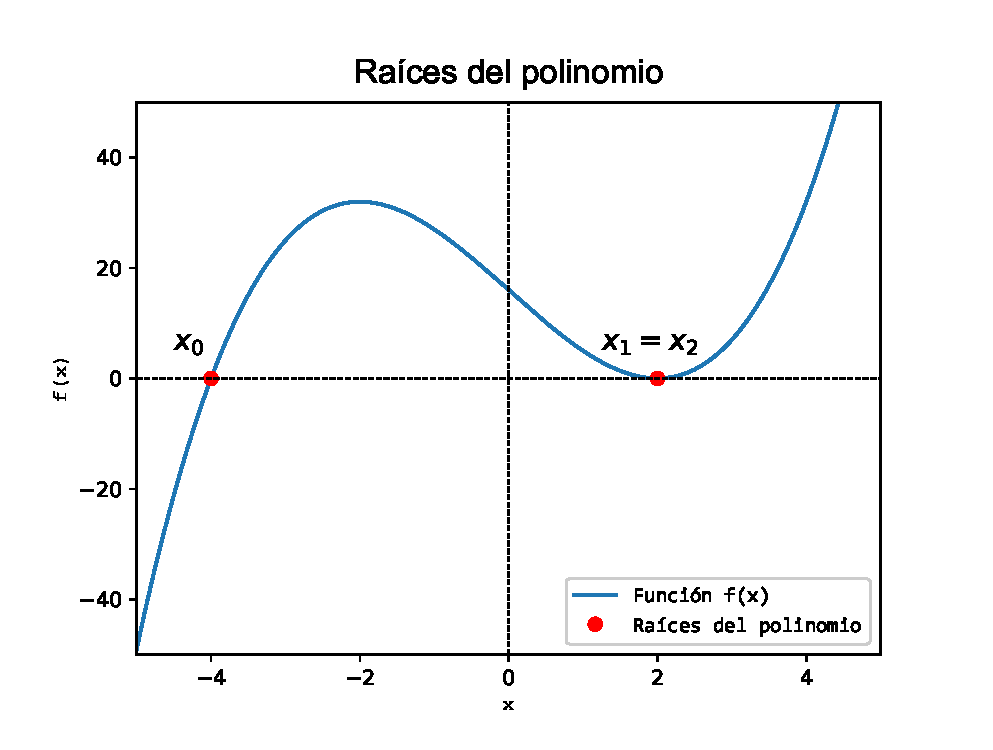
\includegraphics[scale=0.3]{Imagenes/raices_polinomio_2020_03.eps} 
	\caption{Dos valores de las raíces coinciden.}
\end{figure}
\end{minipage}
\end{frame}
\begin{frame}[fragile]
\setbeamerfont{caption}{size=\scriptsize}
\captionsetup{justification=centering}
\frametitle{Raíz real y un par conjugado complejo}
\begin{minipage}{5cm}
\fontsize{12}{12}\selectfont
\begin{align*}
f(x) &= x^{3} - 2 \: x^{2} - 3 \: x + 10  \\
&= (x + 2)(x - (2 + i))* {}\\
&* (x - (2 - i))
\end{align*}
\end{minipage}
\hspace{0.5cm}
\begin{minipage}{5cm}
\begin{figure}
	\centering
	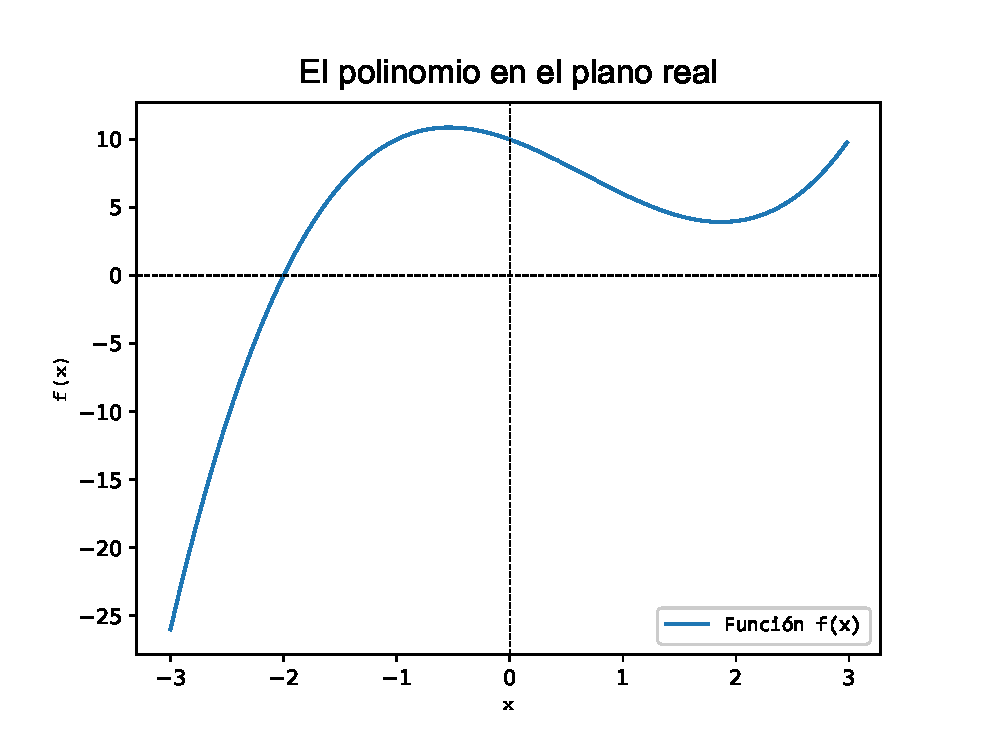
\includegraphics[scale=0.4]{Imagenes/raices_polinomio_2020_04.eps} 
	\caption{La función en el plano real.}
\end{figure}
\end{minipage}
\end{frame}
\begin{frame}[fragile]
\setbeamerfont{caption}{size=\scriptsize}
\captionsetup{justification=centering}
\frametitle{Raíces en el plano de Argand}
\fontsize{12}{12}\selectfont
\begin{minipage}{5cm}
Las raíces son:
\begin{align*}
x_{1} &= -2 \\
x_{2} &= 2 + i \\
x_{3} &= 2 - i \\
\end{align*}
\end{minipage}
\hspace{0.5cm}
\begin{minipage}{5cm}
\begin{figure}
    \centering
    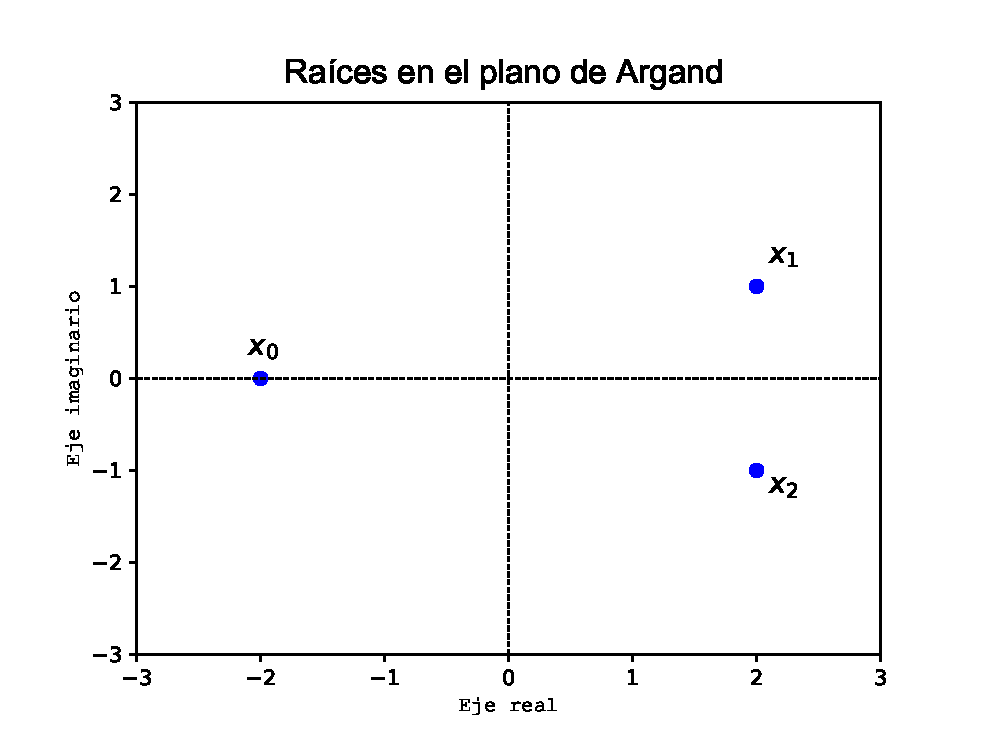
\includegraphics[scale=0.4]{Imagenes/raices_polinomio_2020_05.eps} 
    \caption{Las raíces en el plano de Argand.}
\end{figure}
\end{minipage}
\end{frame}    
\section{Funciones algebraicas y trascendentales}
\frame{\tableofcontents[currentsection, hideothersubsections]}
\subsection{Funciones algebraicas}
\begin{frame}
\frametitle{Funciones algebraicas}
Sea $g = f(x)$ la función expresada como
\[ f_{n} \: y^{n} + f_{n-1} \: y^{n - 1} + \ldots + f_{1} \: y + f_{0} = 0 \]
Donde $f_{i}$ es un polinomio de orden $i$ en $x$.
\end{frame}
\begin{frame}
\frametitle{Funciones algebraicas}
Los polinomios son un caso simple de funciones algebraicas que se representan generalmente como
\[f_{n}(x) = a_{0} + a_{1} \: x + a_{2} \: x^{2}+ \ldots + a_{n} \: x^{n} \]
Donde $n$ es el orden del polinomio.
\end{frame}
\subsection{Funciones trascendentales}
\begin{frame}
\frametitle{Funciones trascedentales}
Son aquellas funciones que no son algebraicas.
\\
\bigskip
Comprenden a las funciones trigonométricas, exponenciales, logarítmicas, entre otras.
\\
\bigskip
\pause
Ejemplos:
\begin{align*}
f(x) &= ln(x^{2} - 1) \\[0.5em]
g(x) &= e^{-0.2 \: x} \sin(3 \: x - 5)
\end{align*}
\end{frame}
\subsection{Calculando las raíces}
\begin{frame}
\frametitle{Calculando las raíces}
Los métodos numéricos estándar para calcular las raíces de una función se clasifican en dos rubros:
\\
\bigskip
\azulfuerte{1.} La determinación de las raíces reales de ecuaciones algebraicas y trascendentales.
\\
\bigskip
\pause
Las técnicas a emplear en estos casos se diseñaron con el fin de encontrar el valor de una raíz simple de acuerdo con un \emph{\textcolor{red}{conocimiento previo}} de su posición aproximada.
\end{frame}
\begin{frame}
\frametitle{Encontrar las raíces}
\azulfuerte{2.} La determinación de todas las raíces reales y complejas de un polinomio, para lo cual los métodos numéricos estén diseñados específicamente para polinomios. 
\\
\bigskip
\pause
Determinan sistemáticamente todas las raíces del polinomio en lugar de hacerlo sólo con una, dada la posición aproximada.
\end{frame}
\section{Estimando el intervalo de las raíces}
\frame{\tableofcontents[currentsection, hideothersubsections]}
\subsection{Método de incrementos sucesivos}
\begin{frame}
\frametitle{Método de incrementos sucesivos}
Podemos aproximar mucho mejor las raíces de una función, cuando la graficamos.
\\
\bigskip
Con una gráfica general de unos cuantos puntos, tendríamos lo necesario para considerar los valores de las raíces.
\end{frame}
\begin{frame}
\frametitle{Método de incrementos sucesivos}
El método de incrementos sucesivos (también llamado de \emph{búsqueda incremental}) es una herramienta útil que podemos adoptar en conjunto con otras estrategias de cálculo de raíces.
\\
\bigskip
Éste método no nos ofrece más que una referencia sobre el intervalo en dónde podría(n) estar la(esas) raíces.
\end{frame}
\begin{frame}
\frametitle{Método de incrementos sucesivos}
La idea básica detrás del método de búsqueda incremental es simple: si el producto de $f(x_{1}) * f(x_{2})$ tiene signo negativo, entonces hay al menos una raíz en el intervalo $[x_{1}, x_{2}]$.
\\
\bigskip
Esto se debe a que $f(x_{1})$ y $f(x_{2})$ tienen signos opuestos.
\end{frame}
\begin{frame}[fragile]
\frametitle{Caso en donde es posible encontrar la raíz}
\begin{figure}
	\centering
	\includestandalone{Figuras/figura_raices_01}
	\caption{Los puntos de la función evaluada en los extremos tienen signos contrarios.}
\end{figure}
\end{frame}
\begin{frame}[fragile]
\frametitle{Caso en donde no es posible encontrar la raíz}
\begin{figure}
	\centering
	\includestandalone{Figuras/figura_raices_02}
	\caption{Los puntos de la función evaluada en los extremos tienen el mismo signo.}
\end{figure}
\end{frame}
\begin{frame}
\frametitle{Cuando hay una raíz}
Si el intervalo es lo suficientemente pequeño, es probable que contenga una sola raíz.
\\
\bigskip
Así, los ceros de $f(x)$ puede ser detectados mediante la evaluación de la función en  intervalos $\Delta \: x$ y mirando cuando se presente un cambio de signo en la función.
\end{frame}
\begin{frame}
\frametitle{Consideraciones con el método}
Hay varios puntos que debemos de considerar con el método de incrementos sucesivos:
\setbeamercolor{item projected}{bg=purple!70!black,fg=white}
\setbeamertemplate{enumerate items}[circle]
\begin{enumerate}[<+->]
\item Es posible perder dos raíces muy próximas entre sí, si el incremento de búsqueda $\Delta \: x$ es mayor que la separación de las raíces.
\\
\bigskip
Por lo que hay que ser cuidados para establecer el valor de $\Delta \: x$.
\seti
\end{enumerate}
\end{frame}
\begin{frame}
\frametitle{Consideraciones con el método}
\setbeamercolor{item projected}{bg=purple!70!black,fg=white}
\setbeamertemplate{enumerate items}[circle]
\begin{enumerate}[<+->]	
\conti
\item Una raíz con multiplicidad doble, es decir: dos raíces que coinciden, no será detectada. Inclusive raíces con multiplicidad triple.
\\
\bigskip
Al considerar el order del polinomio o tipo de función, podemos considerar el número de raíces en el intervalo dado.
\seti
\end{enumerate}
\end{frame}
\begin{frame}
\frametitle{Consideraciones con el método}
\setbeamercolor{item projected}{bg=purple!70!black,fg=white}
\setbeamertemplate{enumerate items}[circle]
\begin{enumerate}[<+->]	
\conti
\item Algunas singularidades de $f(x)$ se puede confundir con raíces. 
\\
\bigskip
Por ejemplo, $f(x) = \tan x$. Tiene cambios de signo en $x = \dfrac{\pi}{2} + n \, \pi$ con $n = 1, 2, 3, 4, \ldots$
\end{enumerate}
\end{frame}
\begin{frame}
\frametitle{Casos en donde no hay una raíz}
\begin{figure}
	\centering
	\includegraphics[scale=0.4]{Imagenes/raices05.eps}
	\caption{Estos puntos no son ceros verdaderos, ya que la función no cruza el eje $x$.}
\end{figure}
\end{frame}
\subsection{Código Método de incrementos sucesivos}
\begin{frame}
\frametitle{Código Método de incrementos sucesivos}
El código en \python{} que presentamos, busca un cero de la función $f(x)$ que proporciona el usuario en el intervalo $(a, b)$, con incrementos de tamaño $dx$, revisando que el producto $f(x_{1})*f(x_{2}) < 0$
\end{frame}
\begin{frame}
\frametitle{Código Método de incrementos sucesivos}
En caso de que se haya detectado un cambio de signo, lo que implica que en el intervalo $(x_{1}, x_{2})$  se encuentra una raíz.
\\
\bigskip
Cuando no se encontraron raíces, es decir, el producto $f(x_{1})*f(x_{2}) > 0$, se devuelve $x_{1} = x_{2} = \mathsf{None}$.
\end{frame}
\begin{frame}
\frametitle{Código Método de incrementos sucesivos}
Luego de que se encontró la primera raíz, (la más cercana al punto $a$), se puede llamar de nuevo al procedimiento, sustitiyendo $x_{2}$ con el fin de encontrar la siguiente raíz. 
\\
\bigskip
Esto se puede repetir siempre y cuando se detecta una raíz.
\end{frame}
\begin{frame}[allowframebreaks, fragile]
\frametitle{Función \azulfuerte{\texttt{buscaraiz}}}
\begin{lstlisting}[caption=Código inicial para buscar los intervalos, style=codigopython]
def buscaraiz(f, a, b, dx):
    xA_1_B = a; fA_1_B = f(a)
    xA_2_B = a + dx; fA_2_B = f(xA_2_B)
    while fA_1_B * fA_2_B > 0.0:
        if xA_1_B >= b: return None
        xA_1_B = xA_2_B; fA_1_B = fA_2_B
        xA_2_B = xA_1_B + dx; fA_2_B = f(xA_2_B)
    else:
        return xA_1_B, xA_2_B
\end{lstlisting}
\end{frame}
\subsection{Ejercicio}
\begin{frame}
\frametitle{Ejemplo para encontrar una raíz}
Usa el método de incrementos sucesivos con espaciamientos de $\Delta x= 0.2$, para estimar la raíz con el valor positivo más pequeño de la función:
\[ f(x) = x^{3} - 10 x^{2} + 5\]
\end{frame}
\begin{frame}
\frametitle{¿Cómo resolver el problema?}
Como el ejercicio pide que se localice la raíz positiva más pequeña, habrá que tener una idea sobre el comportamiento de la función.
\\
\bigskip
Para ello, graficamos en un intervalo inicial, considera que hay potencias al cubo.
\end{frame}
\begin{frame}
\frametitle{Gráfica inicial de la función}
\begin{figure}
	\centering
	\includegraphics[scale=0.5]{Imagenes/aprox_sucesivas_2020_01.eps}
	\caption{De la gráfica vemos que hay tres raíces, la raíz $x{1}$ es la raíz positiva más pequeña.} 
\end{figure}
\end{frame}
\begin{frame}
\frametitle{Acotando el problema}
Como se nos pide el valor de la raíz positiva más pequeña, descartamos las raíz negativa y la otra raíz positiva.
\\
\bigskip
En la siguiente gráfica se reduce el intervalo sobre el eje $x$ para tener una mejor vista.
\end{frame}
\begin{frame}
\frametitle{El intervalo de la gráfica se ha acotado}
\begin{figure}
	\centering
	\includegraphics[scale=0.5]{Imagenes/aprox_sucesivas_2020_02.eps}
	\caption{Se aprecia mucho mejor al reducir el intervalo, pero nos falta aún estimar con el código el intervalo donde está la raíz positiva más pequeña.} 
\end{figure}
\end{frame}
\begin{frame}[fragile]
\frametitle{Ahora con \python}
\begin{lstlisting}[caption=Solución con python, style=codigopython]
def f(x): return x**3 - 10*x**2 + 5.

a, b, dx = (0.0, 1.5, 0.2)

xA_1_B, xA_2_B = buscaraiz(f, a, b, dx)

print('Una raiz esta en el intervalo: ({0:1.2f}, {1:1.2f})'.format(xA_1_B, xA_2_B))
\end{lstlisting}
\end{frame}
\begin{frame}
\frametitle{El intervalo de trabajo}
\begin{figure}
	\centering
	\includegraphics[scale=0.5]{Imagenes/aprox_sucesivas_2020_03.eps}
	\caption{El código devuelve el intervalo de interés, por lo que ahora hay que usar alguna técnica para conocer el valor de la raíz.} 
\end{figure}
\end{frame}
\section{Métodos para el cálculo de raíces}
\frame{\tableofcontents[currentsection, hideothersubsections]}
\subsection{Método de Bisección}
\begin{frame}
\frametitle{Método de Bisección}
Después de que se ha identificado una raíz $f(x) = 0$ en el intervalo $(x_{1}, x_{2})$, disponemos de varios métodos para encontrar el valor de la raíz.
\end{frame}
\begin{frame}
\frametitle{Método de Bisección}
El método de bisección logra esta tarea: \textcolor{red}{el intervalo donde se presume que hay una raíz, se reduce sucesivamente a la mitad  hasta que se vuelve suficientemente pequeño}. 
\end{frame}
\begin{frame}
\frametitle{Método de Bisección}
La técnica de bisección no es el método más rápido disponible, pero es el más fiable.
\\
\bigskip
Una vez que una raíz se ha encontrado en un intervalo, nos podemos acercar a ella.
\end{frame}
\begin{frame}
\frametitle{Funcionamiento del método}
El método de bisección utiliza el mismo principio que el de incrementos sucesivos:
\\
\bigskip
Si hay una raíz en el intervalo $(x_{1}, x_{2})$, entonces revisa si el producto $f(x_{1})*f(x_{2}) < 0$.
\end{frame}
\begin{frame}
\frametitle{Funcionamiento del método}
Con el fin de reducir a la mitad el intervalo, se calcula $f(x_{3})$, donde
\begin{align*}
x_{3} = \dfrac{(x_{1} + x_{2})}{2}
\end{align*}
es el punto medio del intervalo.
\end{frame}
\begin{frame}
\frametitle{Descripción gráfica del método de bisección}
\setbeamercovered{invisible}
\begin{figure}
	\centering
	\includestandalone{Figuras/biseccion_01}
	\caption{Si el producto $f(x_{1})*f(x_{2}) < 0$, entonces se divide el intervalo a la mitad.}
\end{figure}
\end{frame}
\begin{frame}
\frametitle{Funcionamiento del método}
Si $f(x_{1})*f(x_{3}) < 0$, entonces la raíz debe estar en $(x_{1}, x_{3})$ entonces re-emplazamos del intervalo inicial $x_{2}$ por $x_{3}$, y se repite la división del intervalo.
\setbeamercovered{invisible}
\pause
\begin{figure}
	\centering
	\includestandalone{Figuras/biseccion_02}
\end{figure}
\end{frame}
\begin{frame}
\frametitle{Funcionamiento del método}
De lo contrario, la raíz se encuentra en el intervalo $(x_{3}, x_{2})$, en tal caso, se sustituye $x_{3}$ por $x_{1}$, y se repite la división del intervalo.
\end{frame}
\begin{frame}
\frametitle{¿Hasta cuando se repite la división del intervalo?}
En cualquiera de los casos, el nuevo intervalo $(x_{1}, x_{2})$ es la mitad del tamaño del intervalo original.
\\
\bigskip
La bisección es repite hasta que el intervalo se ha reducido a un valor $\varepsilon$ pequeño, de modo que
\begin{align*}
\abs{x_{2} - x_{1}} \leq \varepsilon
\end{align*}
\end{frame}
\begin{frame}
\frametitle{Estimar el número de divisiones del intervalo}
Es fácil calcular el número de bisecciones necesarias para alcanzar el valor de $\varepsilon$.
\\
\bigskip
\pause
El intervalo inicial $\Delta \: x$, se reduce a $\Delta \: x /2$ en la primera bisección, $\Delta \: x /2^{2}$ en la segunda, luego de $n$ bisecciones, $\Delta \: x /2^{n}$.
\\
\bigskip
\pause
Haciendo $\Delta \: x /2^{n} = \varepsilon$, resolvemos para $n$
\begin{align*}
n = \dfrac{\ln(\abs{\Delta x} / \varepsilon)}{\ln 2}
\end{align*}
\end{frame}
\begin{frame}[allowframebreaks, fragile]
\frametitle{Código para el método de bisección}
\begin{lstlisting}[caption=Método de bisección con \python, style=codigopython]
def biseccion(f, xA_1_B, xA_2_B, switch = 0, tol = 1.0e-9):
    fA_1_B = f(xA_1_B)
    if fA_1_B == 0.0: return xA_1_B
    
    fA_2_B = f(xA_2_B)
    if fA_2_B == 0.0: return xA_2_B
    
    if sign(fA_1_B) == sign(fA_2_B):
        print('La raiz no esta en el intervalo')

    n = int(math.ceil(math.log(abs(xA_2_B - xA_1_B)/tol)/math.log(2.0)))
    
    for i in range(n):
        xA_3_B = 0.5 * (xA_1_B + xA_2_B); fA_3_B = f(A_3_B)
        if (switch == 1) and (abs(fA_3_B) > abs(fA_1_B)) \
                    and (abs(fA_3_B) > abs(fA_2_B)):
                        
            return None
        
        if fA_3_B == 0.0: return xA_3_B

        if sign(fA_2_B) != sign(fA_3_B): xA_1_B = xA_3_B; fA_1_B = fA_3_B
        else: xA_2_B = xA_3_B; fA_2_B = fA_3_B
    
    return (xA_1_B + xA_2_B)/2.0
\end{lstlisting}
\end{frame}
\begin{frame}
\frametitle{El argumento \texttt{switch}}
Al establecer el valor del argumento \texttt{switch} $=1$, forzamos la rutina para verificar si la magnitud de $f(x)$ disminuye con cada intervalo a la mitad.
\end{frame}
\begin{frame}
\frametitle{El argumento \texttt{switch}}
Si no lo hace, algo puede estar mal: probablemente la \enquote{raíz}, no es una raíz en absoluto, pero si un polo.
\\
\bigskip
En ese caso, se devuelve \texttt{raíz = None}. Porque esta característica no siempre es deseable, el valor predeterminado es \texttt{switch} $=0$.
\end{frame}
\begin{frame}[fragile]
\frametitle{¿Qué hace la función \azulfuerte{\texttt{ceil}}?}
La función \texttt{ceil} devuelve el menor entero mayor o igual a $x$.
\\
\medskip
Ejemplos:\\
\medskip
\verb|>>>ceil(1.1) # 2.0| \\
\verb|>>>ceil(1.6) # 2.0| \\
\verb|>>>ceil(-1.1) # -1.0| \\
\verb|>>>ceil(-1.6) # -1.0|
\end{frame}
\begin{frame}
\frametitle{Módulo para los métodos}
Con la finalidad de mejorar las técnicas de programación con \python, todas las funciones para calcular las raíces de una función, las almacenaremos en un \emph{Módulo}, al que llamaremos \texttt{ModuloRaices.py}
\end{frame}
\begin{frame}[fragile]
\frametitle{Ejemplo}
Con el método de bisección, calcular la raíz de $f(x)$ que se encuentra en el intervalo $(0,1)$, con una precisión de 4 dígitos
\begin{align*}
f(x) = x^{3} - 10 \; x^{2} + 5 = 0
\end{align*}
\\
\bigskip
¿Cuántas evaluaciones se requieren para encontrar la raíz?
\end{frame}
\begin{frame}[fragile]
\frametitle{Ejemplo}
Como primer punto, generamos una gráfica para tener una idea del comportamiento de la función
\begin{figure}
	\centering
	\includegraphics[scale=0.5]{Imagenes/Ejercicio_4_2_Libro.eps}
\end{figure}
\end{frame}
\begin{frame}[allowframebreaks, fragile]
\frametitle{Solución}
\begin{lstlisting}[caption=Solución al ejercicio, style=codigopython]
from ModuloRaices import biseccion

def f(x): return x**3 - 10.0*x**2 + 5.0

raiz = biseccion(f, 0., 1.0, tol = 1.0e-4)

print('Se tiene un raiz en= ', '{0:1.4f}'.format(raiz))
\end{lstlisting}
\end{frame}
\begin{frame}[fragile]
\frametitle{Solución gráfica}
Una vez calculada la raíz, podemos presentarla en la gráfica
\begin{figure}
	\centering
	\includegraphics[scale=0.4]{Imagenes/Ejercicio_4_2_02_Libro.eps}
\end{figure}
\end{frame}
\begin{frame}
\frametitle{Ejercicio para resolver}
La función
\begin{align*}
f(x) = x^{3} - 10 \; x^{2} + 5 = 0
\end{align*}
tiene tres raíces. ¿Cómo implementamos de manera combinada el método de incrementos sucesivos y el de bisección para calcular las tres raíces?
\end{frame}
\begin{frame}
\frametitle{Ejercicio para resolver}Presenta un código en \python{} que resuelva esta tarea, como sugerencia, identifica el intervalo en donde se presentan las tres raíces.
\end{frame}
% % \begin{frame}[fragile]
% % \frametitle{Algoritmo para el método de bisección}
% % 	\begin{lstlisting}
% %     for i in np.arange(n):
% %         x3 = 0.5*(x1 + x2); f3 = f(x3)
% %         if (switch == 0) and (abs(f3) > abs(f1)) \
% %                         and (abs(f3) > abs(f2)):
% %             return None
% %         if f3 == 0.0: return x3
% %         if f2*f3 < 0.0:
% %             x1 = x3; f1 = f3
% %         else:
% %             x2 =x3; f2 = f3
% %     return (x1 + x2)/2.0
% % 	\end{lstlisting}

% % \end{frame}
\begin{frame}
\frametitle{El argumento \texttt{switch}}
Haciendo que el argumento \texttt{switch} = 1 de la función \funcionazul{biseccion}, se forza la rutina para comprobar si la magnitud de $f(x)$ disminuye con la reducción a la mitad de cada intervalo.
\end{frame}
\begin{frame}
\frametitle{El argumento \texttt{switch}}
Si no es así, algo anda mal (probablemente la \enquote{raíz} no es una raíz en absoluto, sino una singularidad) y se devuelve la \texttt{raíz} = \texttt{None}.
\\
\bigskip
Dado que esta característica no siempre es deseable, el valor predeterminado es \texttt{{switch} = 0}.
\end{frame}
\begin{frame}
\frametitle{El argumento \texttt{switch}}
Veamos lo que hace la variable \texttt{switch}:
\\
\medskip
Hasta el momento no nos hemos fijado en la magnitud de $f(x_{1})$ y $f(x_{2})$, sólo en el signo del respectivo producto, 
\end{frame}
\begin{frame}
\frametitle{El argumento \texttt{switch}}
Ahora tomamos en cuenta la magnitud tanto de los puntos evaluados en la función como del producto mismo.
\\
\medskip
Consideremos el primer caso de la función $f(x)$, donde ya sabemos que hay una raíz en el intervalo $[0.6, 0.8]$
\end{frame}
\begin{frame}[fragile]
\frametitle{El valor por defecto de \texttt{switch} = 0}
\begin{tabular}{l | l | l |  l | l | l}
$x_{1}$ & $x_{2}$ & $f(x_{1})$ & $f(x_{2})$ & $f(x_{1})f(x_{2})$ & signo \\ \hline
$0.0$ & $0.2$ & $5.000$ & $4.608$ & $23.0400$ & $+1$ \\ \hline
$0.2$ & $0.4$ & $4.608$ & $3.464$ & $15.9621$ & $+1$ \\ \hline
$0.4$ & $0.6$ & $3.464$ & $1.616$ & $5.5978$ & $+1$ \\ \hline
$0.6$ & $0.8$ & $1.616$ & $-0.888$ & $-1.4350$ & $+1$ \\ \hline
$0.8$ & $1.0$ & $-0.888$ & $-4.000$ & $3.5520$ & $-1$ \\ \hline
$1.0$ & $1.2$ & $-4.000$ & $-7.672$ & $30.688$ & $+1$
\end{tabular}
% \begin{tikzpicture}[overlay]
%Define the circle paths
	% \draw [blue](1.north west) -- (1.north east) -- (2.south east) -- (2.south west) -- cycle;
	%\draw [red](3.north west) -- (3.north east) -- (4.south east) -- (4.south west) -- cycle;
% \end{tikzpicture}
\end{frame}
\begin{frame}
\frametitle{Magnitud del producto}
Vemos que conforme avanza el desplazamiento en el intervalo $x_{1}$ y $x_{2}$, la magnitud del producto $f(x_{1}) * f(x_{2})$ también va cambiando.
\\
\bigskip
Lo importante es también el signo del producto, al llegar al intervalo donde hay cambio de signo, la magnitud del producto es la mínima, en el siguiente paso, se incrementa nuevamente.
\end{frame}
% \begin{frame}[fragile]
% \frametitle{Revisión del código}
% Del código tenemos que:
% \begin{verbatim}
% if (switch == 1) and (abs(f3) > abs(f1)) \ 
%                  and (abs(f3) > abs(f2)):
%     return None
% \end{verbatim}
% \end{frame}
% \begin{frame}[fragile]
% \frametitle{Revisión del código}
% Revisando para el primer renglón con los valores de la tabla:
% \begin{tabular}{l | l | l}
% $abs(f3) > abs(f1)$ & $abs(f3) > abs(f2)$ & Expresión \\ \hline
% \texttt{True} & \texttt{True} & True \\ \hline

% \end{tabular}
% Aquí tendrán que completar la tabla de tal manera que revisen el resultado de la expresión compuesta.
% \end{frame}
\begin{frame}
\frametitle{Ejercicios para entregar}
Determina el(los) intervalo(s) en donde se localizan todas las raíces y usando el método de bisección calcula la(s) raíz(ces) de:
\begin{align*}
f(x) &= x^{3} - 10 \, x^{2} + 5 \\[0.5em]
g(x) &= x - \tan(x) \hspace{1cm} 0 \leq x \leq 20
\end{align*}
Con una tolerancia de $\num{d-9}$
\end{frame}
\begin{frame}
\frametitle{Consideraciones previas}
\setbeamercolor{item projected}{bg=blue!70!black,fg=yellow}
\setbeamertemplate{enumerate items}[circle]
\begin{enumerate}[<+->]
\item Toma en cuenta que $\tan(x)$ es singular y cambia de signo en $x = \pi/2, 3\pi/2,\ldots$. Para no unir estos puntos para las raíces, hacemos \texttt{switch}= 1.
\item La proximidad de las raíces a las singularidades es otro problema potencial que puede ser prevenido ante el uso de $\Delta x$ pequeña, usa $x = 0.01$.
\end{enumerate}
\end{frame}
\begin{frame}
\frametitle{Graficas de las funciones y sus raíces}
\begin{figure}
	\centering
	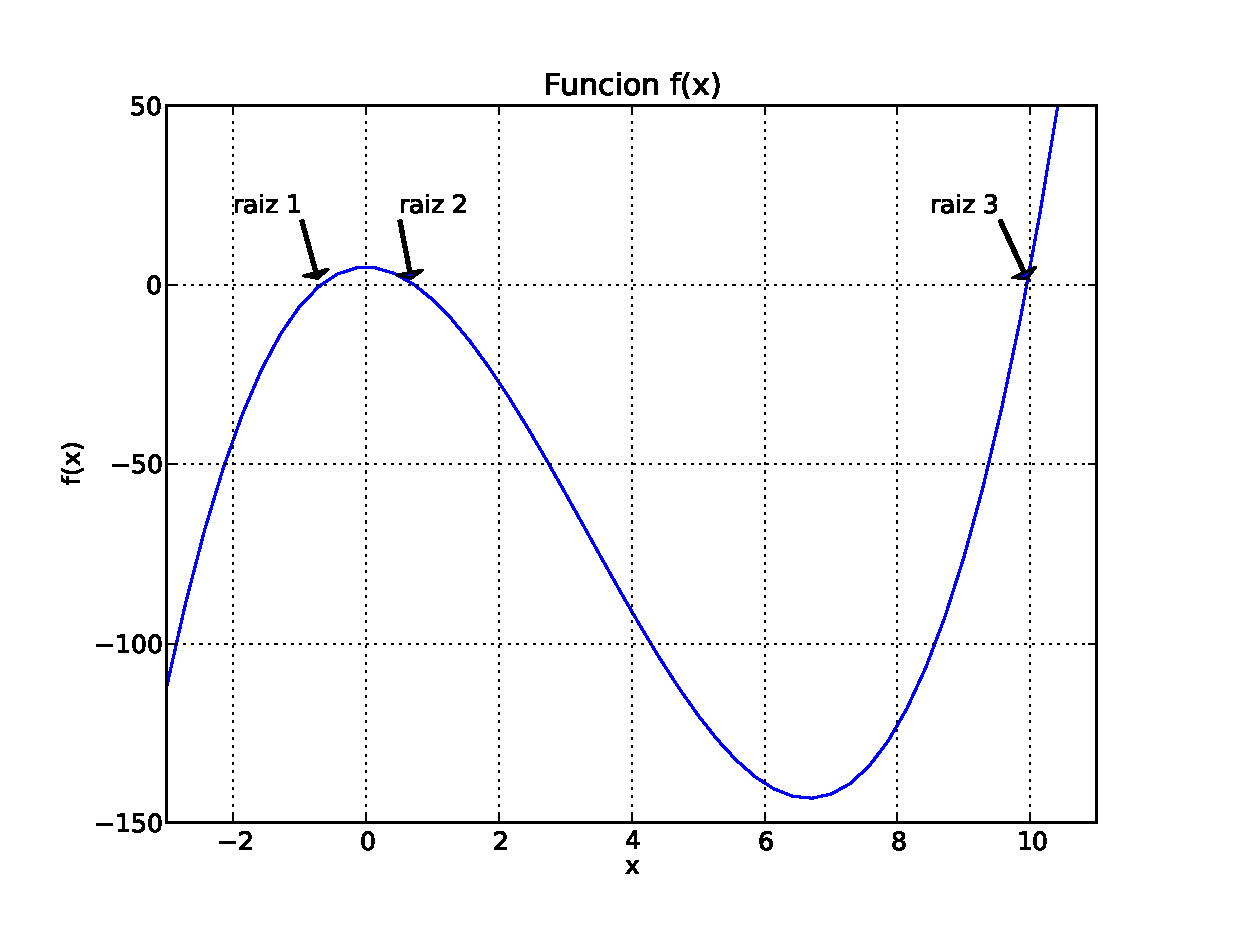
\includegraphics[scale=0.4]{Imagenes/ejercicio1_Biseccion.eps}<1>
	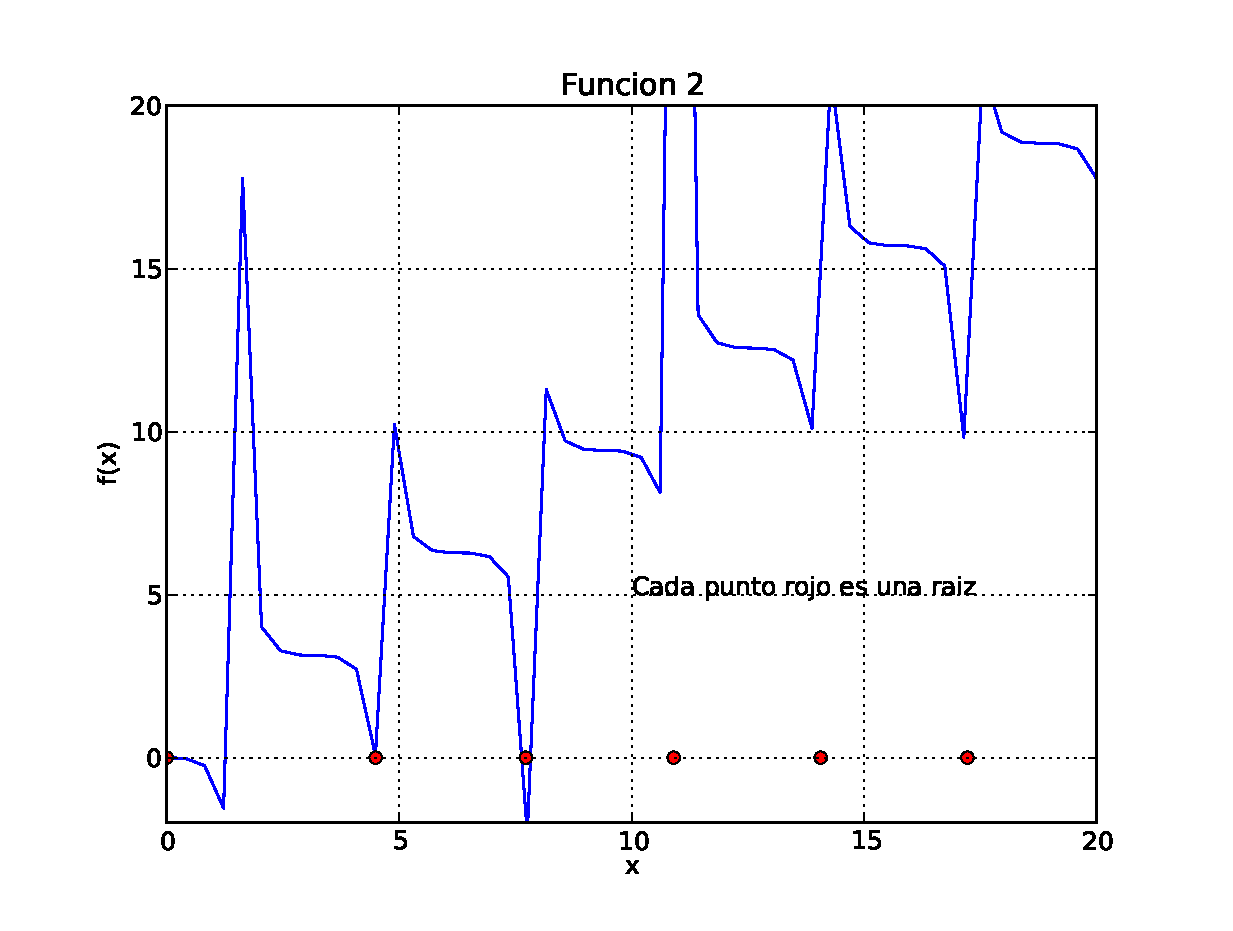
\includegraphics[scale=0.4]{Imagenes/ejercicio2_Biseccion.eps}<2>
\end{figure}
\end{frame}
% \begin{frame}
% \frametitle{Estrategia de solución}
% Para integrar los elementos que hemos visto:
% \begin{enumerate}
% \item Recuperamos el algoritmo que nos identifica en qué intervalo se encuentra una raíz.
% \item Aplicamos el algoritmo del método de bisección.
% \item Usamos un ciclo que nos revise en el dominio que se nos proporciona, si existe más de una raíz.
% \end{enumerate}
% \end{frame}
% % \begin{frame}[fragile]
% % \begin{lstlisting}
% % def f(x): return x**3-10*x**2+5

% % a,b,dx = (-2.0,11.0,0.02)
	
% % print 'Intervalo (x1,x2)   raiz'
% % while 1:
% %     try:
% %         x1, x2 = buscaraiz(f,a,b,dx)
% %     except Exception, e:
% %         print e; break
% %     if x1 != None:
% %         a = x2
% %         root = bisect(f,x1,x2,0)
% %         if raiz != None: print '(%2.4f, %2.4f) %2.8f' %(x1, x2, raiz)
% % \end{lstlisting}
% % \end{frame}
% % \begin{frame}[fragile]
% % \begin{lstlisting}
% %     else:
% %         print '\nHecho'
% %         break
% % \end{lstlisting}
% % \end{frame}
\subsection{Método de Newton-Raphson}
\begin{frame}
\frametitle{Método de Newton-Raphson}
El método de Newton-Raphson es el algoritmo más conocido para encontrar raíces por una buena razón: es simple y rápido.
\\
\medskip
El único detalle es que utiliza una función $f(x)$ y su derivada de primer orden $f^{\prime}(x)$.
\end{frame}
\begin{frame}
\frametitle{Método de Newton-Raphson}
Por tanto, en los problemas a resolver con este algoritmo, deberá de contemplarse que la derivada sea fácil de calcularse (a mano).
\end{frame}
\begin{frame}
\frametitle{Método de Newton-Raphson}
El método de Newton-Raphson (N-R) se obtiene de la expansión en series de Taylor de $f(x)$ alrededor de $x$:
\begin{align*}
f(x_{i + 1})  = f(x_{i}) + f^{\prime}(x_{i})(x_{i + 1} - x_{i}) + \order{x_{i + 1} - x_{i}}^{2}
\end{align*}
\end{frame}
\begin{frame}
\frametitle{Método de Newton-Raphson}
Si $x_{i + 1}$ es una raíz de $f(x) = 0$, tenemos que:
\begin{align*}
0 = f(x_{i}) + f^{\prime}(x_{i})(x_{i + 1} - x_{i}) + \order{x_{i + 1} - x_{i}}^{2}
\end{align*}
Suponiendo que $x_{i}$ está cerca de $x_{i + 1}$, podemos eliminar el último término de la ecuación y resolver para $x_{i+1}$:
\end{frame}
\begin{frame}
\frametitle{Método de Newton-Raphson}
Por lo que la fórmula de Newton-Raphson es:
\begin{align*}
x_{i+1} = x_{i} - \dfrac{f(x_{i})}{f^{\prime}(x_{i})}
\end{align*}
\end{frame}
\begin{frame}
\frametitle{Método de Newton-Raphson}
Si $x$ representa el valor verdadero de la raíz, el error en $x_{i}$ es $E_{i} = x - x_{i}$.
\\
\bigskip
Se puede demostrar que si $x_{i+1}$ se calcula de la expresión de N-R, el error es:
\begin{align*}
E_{i+1} = - \dfrac{f^{\prime \prime}(x_{i})}{2 \: f^{\prime}(x_{i})} \; E_{i}^{2}
\end{align*}
\end{frame}
\begin{frame}
\frametitle{Método de Newton-Raphson}
Lo que nos dice que el método de N-R converge de manera cuadrática, es decir, el error es el cuadrado del error del punto previo.
\end{frame}
\begin{frame}[fragile]
\frametitle{Representación gráfica}
Podemos interpretar que $x_{i+1}$ es el punto en donde la tangente de $f(x_{i})$ cruza el eje de las $x$:
\begin{center}
	\begin{tikzpicture}[font=\small, scale=0.8]
		\draw [->] (0,0) -- (7,0);
		\draw [<->] (0,-3) -- (0,3);
		\draw [red, thick] (1,3) .. controls (1.5,0.5) and (5,-2) .. (6.5,-2);
		\draw (1,-0.3) node {$x_{i}$};
		\draw (1,3.3) node {$f(x_{i})$};
		\draw [dashed] (1.2,0) -- (1.2,2.35);
		\draw (0.8,3.1) -- (2.35,-0.1);
		\draw [dashed] (2.3,0) -- (2.3,0.58);
		\draw (2.3,-0.3) node {$x_{i+1}$};
	\end{tikzpicture}
\end{center}
\end{frame}
\begin{frame}[fragile]
\frametitle{Método de Newton-Raphson}
El método de N-R es sencillo: se aplica la expresión para $x_{i + 1}$ iniciando con un valor $x_{0}$, hasta alcanzar un criterio de convergencia:
\begin{align*}
\abs{x_{i+1} - x_{i}} < \varepsilon
\end{align*}
\end{frame}
\begin{frame}[fragile]
\frametitle{Algoritmo Método de Newton-Raphson}
El algoritmo es el siguiente:
\setbeamercolor{item projected}{bg=red!70!black,fg=white}
\setbeamertemplate{enumerate items}[circle]
\begin{enumerate}[<+->]
\item Sea $x$ un valor inicial para la raíz de $f(x) = 0$.
\item Calcular $\Delta x = - f(x)/f^{\prime}(x)$.
\item Asignar $x \leftarrow x + \Delta x$ y se repiten los pasos 2-3, hasta alcanzar $\vert \Delta x \vert < \varepsilon$.
\end{enumerate}
\end{frame}
\begin{frame}[fragile]
\frametitle{Precaución con el método N-R}
Aunque el método de Newton-Raphson converge rápidamente cerca de la raíz, sus características globales de convergencia son pobres. 
\\
\bigskip
La razón es que la línea tangente no es siempre una aproximación aceptable de la función.
\end{frame}
\begin{frame}[fragile]
\frametitle{Precaución con el método N-R}
\begin{center}
	\begin{tikzpicture}[font=\small, scale=0.8]
		\draw [->] (0,0) -- (4,0);
		\draw [<->] (0,-1) -- (0,3);
		\draw [red, thick] (1,3) .. controls (2,3) and (2.5,2) .. (3.5,-2);
		\draw (1.2,3) circle (0.05);
		\draw [blue, ->] (1.2,3) -- (3.5,2.7);
		\draw (4.2,0) node {$x$};
		\draw (-0.5,2) node {$f(x)$};
		\draw [dashed] (1.2,0) -- (1.2,3);
		\draw (1.2,-0.2) node {$x_{0}$};
	\end{tikzpicture}
	\captionof{figure}{La recta tangente no se aproxima a la función.}
\end{center}
\end{frame}
\begin{frame}[fragile]
\frametitle{Precaución con el método N-R}
\begin{center}
\setbeamercovered{invisible}
	\begin{tikzpicture}%[decoration={markings,% activar las marcas	mark= at position 2cm with{\arrow{stealth}}}]
		\draw [->] (0,0) -- (6,0);
		\draw [<->] (0,-2) -- (0,2);
		\draw [red, thick] (0.5,-2) .. controls (3,-1.9) and (3,1.9) .. (5.5,2);
		\draw (4.5,-0.3) node {$x_{0}$};\pause
		\draw [dashed] (4.5,0) -- (4.5,1.69);
		\draw (4.5,1.7) circle (0.04);
		\draw [blue, postaction={decorate}] (4.5,1.7) -- (1,0);
		\draw (1,0.3) node {$x_{1}$};
		\draw (1,0) circle (0.04);\pause
		\draw [dashed] (1,0) -- (1,-1.95);
		\draw (1,-1.95) circle (0.04);
		\draw [blue,, postaction={decorate}] (1,-1.95) -- (5.8,0.1);
	\end{tikzpicture}
	\captionof{figure}{\only<1>{Consideremos está función \enquote{sigmoidea}.}\only<2>{Se tiende la tangente y se estima $x_{1}$ para luego evaluar $f(x_{1})$.}\only<3>{La tangente nos regresa de nuevo al punto inicial, se tendría un bucle infinito del que no saldríamos.}}
\end{center}
\end{frame}
% \subsection{Algoritmo para el método Newton-Raphson}
\begin{frame}
\frametitle{Algoritmo para el método Newton-Raphson}
La siguiente algoritmo para el método de Newton-Raphson supone que la raíz a calcularse inicialmente está en el intervalo (a, b).
\\
\bigskip
Ese intervalo se habría obtenido del algoritmo de incrementos sucesivos.
\end{frame}
\begin{frame}
\frametitle{Algoritmo para el método Newton-Raphson}
El punto medio del intervalo se utiliza como aproximación inicial de la raíz. Los extremos del intervalo se actualizan luego de cada iteración.
\\
\bigskip
Si una iteración del método Newton-Raphson no se mantiene dentro del intervalo, se descarta y se reemplaza con el método de bisección.
\end{frame}
\begin{frame}
\frametitle{Algoritmo para el método Newton-Raphson}
El método \funcionazul{newtonRaphson} utiliza la función $f(x)$, así como su derivada, (denotadas por $f$ y $df$) deben ser proporcionadas por el usuario.
\end{frame}
\begin{frame}[plain, allowframebreaks, fragile]
\frametitle{Algoritmo de \texttt{Newton-Raphson}}
\begin{lstlisting}[caption=Código del método N-R, style=codigopython]
def newtonRaphson(f, df, a, b, tol = 1.0e-9):
    fa = f(a)
	if fa == 0.0: return a

    fb = f(b)
    if f(b) == 0.0: return b

   if fa*fb>0.0: print('La raiz no esta en el intervalo')

	x = 0.5 * (a + b)

   for i in range(30):
      fx = f(x)
      if abs(fx) < tol: return x

      if fa*fx < 0.0:
         b = x
      else:
         a = x; fa = fx

      dfx = df(x)
        
      try: dx = -fx/dfx
      except ZeroDivisionError: dx = b - a
      x =  x + dx
  
      if(b - x)*(x - a) < 0.0:
         dx = 0.5*(b-a)
         x = a + dx
        
      if abs(dx) < tol*max(abs(b),1.0): return x
    
   print('Son demasiadas iteraciones')
\end{lstlisting}
\end{frame}
\begin{frame}
\frametitle{Responde las preguntas}
\setbeamercolor{item projected}{bg=blue!70!black,fg=yellow}
\setbeamertemplate{enumerate items}[circle]
\begin{enumerate}[<+->]
\item ¿Por qué tenemos una secuencia de iteración de 30 elementos? ¿Por qué no 20 ó 50?
\item Explica el uso de la excepción: ¿en qué caso se podría presentar la división entre cero?
\end{enumerate}
\end{frame}
\begin{frame}
\frametitle{Ejercicio}
Calcula la raíz positiva más pequeña de la función:
\begin{align*}
f(x) = x^{4} - 6.4 \, x^{3} + 6.45 \, x^{2} + 20.538 \, x - 31.752
\end{align*}
\end{frame}
\begin{frame}
\frametitle{Solución al ejercicio}
Como primer paso: generamos una gráfica de la función $f(x)$:
\begin{figure}
   \centering
   \includegraphics[scale=0.4]{Imagenes/raices_NR_2020_01.eps}
   \caption{Se indican las raíces del polinomio ¿falta alguna?}
\end{figure}
\end{frame}
\begin{frame}
\frametitle{Aclaración sobre las raíces}
De acuerdo con la gráfica de $f(x)$ de la diapositiva anterior, se presentan sólo dos raíces: \emph{¿qué pasó?}
\\
\bigskip
Demuestra a partir de la expresión de $f(x)$ que tiene una raíz con multiplicidad doble.
\end{frame}
\begin{frame}
\frametitle{Un inconveniente para la solución}
También vemos de la gráfica anterior que la raíz positiva más pequeña está cerca del valor $x=2$.
\\
\bigskip
El método de bisección no funcionaría debidamente ya que éste depende del cambio de signo de la función cerca de la raíz.
\end{frame}
\begin{frame}
\frametitle{Alternativa a la solución}
Haremos una versión más sencilla del método \funcionazul{newtonRaphson} que se mostró anteriormente.
\\
\bigskip
Además de mostrar el valor de la raíz, también se indica el número de iteraciones realizadas.
\end{frame}
\begin{frame}[allowframebreaks, fragile]
\frametitle{Código alternativo}
\begin{lstlisting}[caption=Código modificado del método N-R, style=codigopython]
def f(x): return x**4 - 6.4*x**3 + 6.45*x**2 + 20.538*x - 31.752
def df(x): return 4.0*x**3 - 19.2*x**2 + 12.9*x + 20.538
   
def newtonRaphsonA_1_B(x, tol=1e-09):
   for i in range(30):
      dx = -f(x)/df(x)
      x = x + dx
      if abs(dx) < tol: return x, i
   print('Son demasiadas iteraciones\n')

raiz, numIter = newtonRaphsonA_1_B(2.0)

print('Raiz = {0:}'.format(raiz))
print('Numero de iteraciones = {0:d}'.format(numIter))
\end{lstlisting}
\end{frame}
\begin{frame}[fragile]
\frametitle{Resultado obtenido}
Con la modificación del método N-R, tenemos que el valor de la raíz es:
\begin{verbatim}
Raiz = 2.0999999786199406
Numero de iteraciones = 22
\end{verbatim}
\pause
Siendo el valor exacto de la raíz: $x = 2.1$
\end{frame}
\begin{frame}[fragile]
\frametitle{Convergencia del método}
Se puede demostrar que cerca de una raíz múltiple, la convergencia del método N-R es lineal más que cuadrática, lo que explica el número elevado de iteraciones.
\end{frame}
\begin{frame}
\frametitle{Convergencia del método}
Se puede mejorar la velocidad de convergencia del método N-R para el caso de raíces múltiples, haciendo el ajuste:
\begin{align*}
x_{i+1} = x_{i} - m \, \dfrac{f(x_{i})}{f^{\prime}(x_{i})}
\end{align*}
donde $m$ es la multiplicidad de la raíz.
\\
\bigskip
Llama a este programa ajustado como \funcionazul{newtonRaphson3}.
\end{frame}
\begin{frame}
\frametitle{¿Si hay mejora en la convergencia?}
Realiza el ajuste al código de \python{} para calcular: el error relativo (comparado con la versión previa), así como el número de iteraciones que se requieren para el mismo ejercicio.
\\
\bigskip
Este es un ejercicio que hay que responder.
\end{frame}
\begin{frame}
\frametitle{Completa la tabla}
\begin{table}
	\centering
	\begin{tabular}{l | l | l | l}
		Programa & Raíz & Iteraciones & Error relativo \\ \hline
		newtonRaphson2 & & & \\ \hline
		newtonRaphson3 & & & \\ \hline
	\end{tabular}
\end{table}
\end{frame}
\begin{frame}
\frametitle{Siguiente ejercicio}
Usando el método de Newton-Raphson, calcula las dos raíces de la función:
\begin{align*}
f(x) = \sin \: x + 3 \: \cos \: x - 2 = 0
\end{align*}
en el intervalo $(-2, 2)$
\end{frame}
\begin{frame}
\frametitle{Primer paso: graficar la función}
La gráfica de la función en el intervalo dado es la siguiente:
\begin{figure}
	\centering
	\includegraphics[scale=0.5]{Imagenes/Ejercicio_NR_Seno_01.eps}
\end{figure}
\end{frame}
\begin{frame}[fragile]
\frametitle{Llamando a paquetes y módulos}
Será necesario utilizar el módulo \funcionazul{ModuloRaices} que ya tenemos así como el paquete \funcionazul{numpy} y para graficar, la librería \funcionazul{matplotlib.pyplot}
\begin{lstlisting}[caption=Llamada a paquetes y funciones, style=codigopython]
from ModuloRaices import buscaraiz, newtonRaphson
import numpy as np
import matplotlib.pyplot as plt
\end{lstlisting}
\end{frame}
\begin{frame}[fragile]
\frametitle{Intervalos de las raíces}
Con el método de incrementos sucesivos, estimamos cada intervalo donde se encuentran las raíces de la función.
\\
\bigskip
Usaremos dos listas para almacenar los valores de los intervalos; cuando se halla un cambio de signo, entonces se renombra el extremo para continuar la búsqueda de otro intervalo.
\end{frame}
\begin{frame}[allowframebreaks, fragile]
\frametitle{Intervalos de las raíces}
\begin{lstlisting}[caption=Intervalos para las raíces, style=codigopython]
inicio, final, dx = -2., 2. , 0.01

aA_1_B, bA_1_B = buscaraiz(f, inicio, final, 0.1)
print('Una raiz esta en  el intervalo [ {0:1.2f}, {1:1.2f}]'.format( aA_1_B, , bA_1_B))

inicio = bA_1_B

aA_2_B, bA_2_B = buscaraiz(f, inicio, final, 0.1)
print('Una raiz esta en  el intervalo [ {0:1.2f}, {1:1.2f}]'.format( aA_2_B, , bA_2_B))
\end{lstlisting}
\end{frame}
\begin{frame}[fragile]
\frametitle{Los intervalos}
El resultado que nos devuelve la función de incrementos sucesivos es:
\begin{verbatim}
Una raíz está en [ -0.6 , -0.5 ]
Una raíz está en [ 1.2 , 1.3 ]
\end{verbatim}
\end{frame}
\begin{frame}
\frametitle{Calculando las raíces}
La siguiente parte es calcular las raíces con la función \funcionazul{newtonRaphson}, debemos de incluir la función $f(x)$ y su derivada de primer orden $df(x)$, siendo sencillo su cálculo a mano.
\end{frame}
\begin{frame}[allowframebreaks, plain, fragile]
\frametitle{Código completo}
\begin{lstlisting}[caption=Intervalos para las raíces, style=codigopython]
def f(x): return np.sin(x) + 3 * np.cos(x) - 2
def df(x): return np.cos(x) - 3 * np.sin(x)

intervaloA_1_B = []
intervaloA_2_B = []

inicio, final, dx = -2., 2. , 0.01

aA_1_B, bA_1_B = buscaraiz(f, inicio, final, 0.1)
print('Una raiz est en [', round(aA_1_B, 2), ',', round(bA_1_B, 2) , ']')
intervaloA_1_B.append(aA_1_B)
intervaloA_1_B.append(bA_1_B)

inicio = bA_1_B
aA_2_B, bA_2_B = buscaraiz(f, inicio, final, 0.1)
print('Una raiz esta en [', round(aA_2_B,2), ',', round(bA_2_B,2), ']')
intervaloA_2_B.append(aA_2_B)
intervaloA_2_B.append(bA_2_B)

raizA_1_B = newtonRaphson(f, df, intervaloA_1_B[0], intervaloA_1_B[-1], 1.e-4)
print(raizA_1_B)

raizA_2_B = newtonRaphson(f, df, intervaloA_2_B[0], intervaloA_2_B[-1], 1.e-4)
print(raizA_2_B)
\end{lstlisting}
\end{frame}
\begin{frame}[allowframebreaks, plain, fragile]
\frametitle{Rutina de graficación}
Con los resultados obtenidos, procedemos a graficar la función y las raíces.
\begin{lstlisting}[caption=Gráfica con las raíces, style=codigopython]
x = np.linspace(-2,2)

plt.axhline(y=0, ls='dashed', lw=0.7, color='k')
plt.plot(x, f(x), color='g')
plt.plot(raizA_1_B, 0, 'ro', label='Raiz A_1_B = ' + str(round(raizA_1_B, 3)))
plt.plot(raizA_2_B, 0, 'bo', label='Raiz A_2_B = ' + str(round(raizA_2_B, 3)))
plt.legend(loc='lower right')
plt.title('Grafica que muestra dos raices de la funcion')
plt.show()
\end{lstlisting}    
\end{frame}
\begin{frame}
\frametitle{Solución}
La gráfica de la función en el intervalo dado es la siguiente:
\begin{figure}
	\centering
	\includegraphics[scale=0.4]{Imagenes/Ejercicio_NR_Seno_02.eps}
	\caption{Implementando varias etapas, se calcularon las raíces de la función en el  intervalo.}
\end{figure}
\end{frame}
% \begin{frame}
% \frametitle{Ejercicio}
% Encontrar la raíz positiva más pequeña de
% \[ f(x) = x^{4} - 6.4 \: x^{3} + 6.45 \: x^{2} + 20.538 \: x - 31.752\]
% Como en los ejercicios anteriores, es buena idea generar una gráfica de la función.
% \end{frame}
% \begin{frame}
% \frametitle{Gráfica del ejercicio}
% \begin{figure}
% 	\centering
% 	\visible<2-> {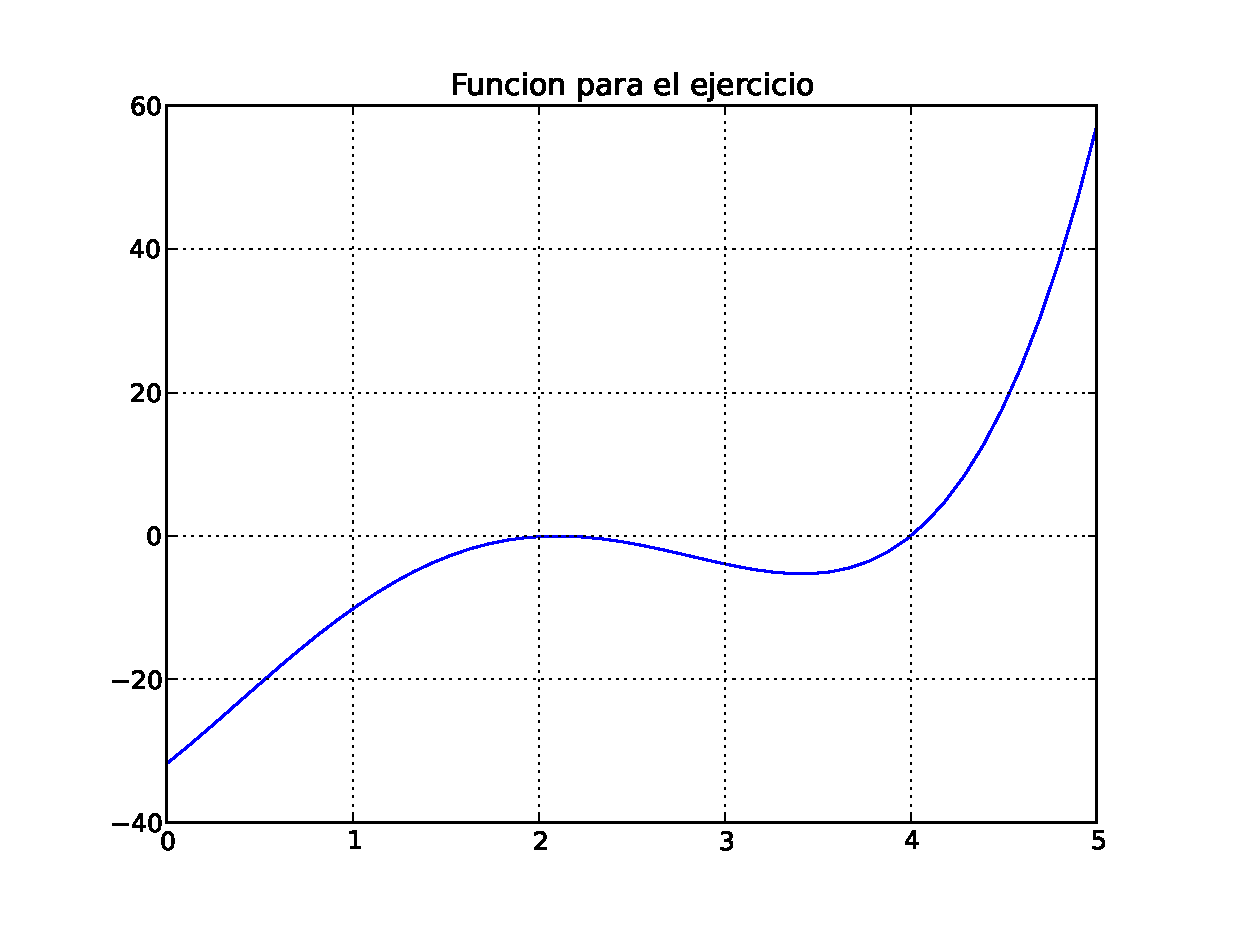
\includegraphics[scale=0.5]{Imagenes/raices08.eps}}
% \end{figure}
% \end{frame}
% \begin{frame}
% \frametitle{Caso particular para esta función}
% Al realizar un poco de álgebra, nos encontramos con lo siguiente:
% \[ 0.002 (x - 4.) (5. x + 9.) (10. x - 21.)^{2} \]
% La función tiene dos raíces reales y una de multiplicidad $2$.
% \end{frame}
% \begin{frame}
% \frametitle{Ajuste al código de NR}
% Como el método de NR se basa en detectar el cambio de signo en la función, en este caso, para una raíz con multiplicidad $2$, haremos un ajuste al código del método.
% \end{frame} 	
% \begin{frame}[allowframebreaks,plain, fragile]
% \frametitle{Ejercicio}
% \begin{lstlisting}[caption=Código para el ejercicio, style=FormattedNumber, basicstyle=\linespread{1.1}\ttfamily=\small, columns=fullflexible]
% def f(x): return x**4 - 6.4*x**3 + 6.45*x**2 + 20.538*x - 31.752
% def df(x): return 4.0*x**3 - 19.2*x**2 + 12.9*x + 20.538

% def newtonRaphson(x,tol=1e-09):
%     for i in range(30):
%         dx = -f(x)/df(x)
%         x = x + dx
%         if abs(dx) < tol: return x,i
%     print 'Son demasiadas iteraciones\n'

% raiz,numIter = newtonRaphson(2.0)

% print 'Raiz =',raiz
% print 'Numero de iteraciones =',numIter
% \end{lstlisting}
% \end{frame}
% \begin{frame}
% \frametitle{Convergencia del método}
% Se puede demostrar que la convergencia del método NR cerca de una raíz con multiplicidad es linear, más que cuadrática.
% \\
% \bigskip
% \pause
% La convergencia de una raíz múltiple se puede acelerar al cambiar la fórmula de NR.
% \end{frame}
% \begin{frame}
% \frametitle{Ajuste a la función NR}
% Se ajusta de la forma
% \[ x_{i + 1} = x_{i} - m \; \dfrac{f(x_{i})}{f^{\prime}(x_{i})} \]
% donde $m$ es la multiplicidad de la raíz (en el ejemplo, $m = 2$). Después de hacer los ajustes, el resultado se obtiene en $5$ iteraciones.
% \end{frame}
% \begin{frame}
% \frametitle{Solución del ejercicio}
% \begin{figure}
% 	\centering
% 	\includegraphics[scale=0.5]{Imagenes/Raiz_NR_02.eps}
% \end{figure}
% \end{frame}
\begin{frame}
\frametitle{Ejercicios para practicar}
Deberán de entregar un archivo por cada uno de los cuatro incisos (incluyendo gráficas):
\begin{enumerate}
\item Encuentra las raíces de
\begin{align*}
x \sin x + 3 \, \cos x - x = 0 \hspace{0.25cm} \text{en } (-6,6)
\end{align*} \\
\item Calcula todas las raíces reales de
\begin{align*}
x^{4} + 0.9\, x^{3} - 2.3 \,x^{2} + 3.6 \, x - 25.2 = 0
\end{align*}
\seti
\end{enumerate}
\end{frame}
\begin{frame}
\frametitle{Ejercicios para practicar}
\begin{enumerate}
\conti
\item Calcula todas las raíces reales de
\begin{align*}
x^{4} + 2 \, x^{3} - 7 \, x^{2} + 3 = 0
\end{align*} \\
\item Calcula todas las raíces de
\begin{align*}
\sin x - 0.1 \, x = 0
\end{align*}
\end{enumerate}
Revisa la pertinencia de utilizar el método N-R o el de bisección. Justifica tu respuesta.
\end{frame}
\subsection{Método de la falsa posición}
\begin{frame}
\frametitle{Método de la falsa posición}
El método de la posición falsa (\emph{regula falsi} o método de regla falsa) tiene como objetivo encontrar una raíz real $\xi$ de una función $f (x) = 0$ que se encuentra en un intervalo [a, b], en donde el producto de la función evaluada en los extremos es de signo contrario: $f(a) * f(b) < 0)$.
\end{frame}
\begin{frame}
\frametitle{Método de la falsa posición}
La principal diferencia con el método de bisección consiste en la forma de elegir los intervalos: $[a_{1}, b_{1}], [a_{2}, b_{2}], \ldots , [a_{i}, b_{i}]$, que en el método de posición falsa no resultan por bisección, sino al dividir el intervalo actual $[a_{i}, b_{i}]$ en la relación $f(a_{i}) / f(b_{i})$ de los valores de la función en los dos extremos.
\end{frame}
\begin{frame}
\frametitle{Método de la falsa posición}
Este procedimiento se repite en una secuencia de pasos de prueba y error, sustituyendo los valores de prueba \enquote{falsos} por las cantidades desconocidas para encontrar aproximaciones sucesivamente mejoradas de la solución.
\end{frame}
\begin{frame}
\frametitle{La geometría del método}
Veamos en las siguientes figuras la manera en que funciona el método de la falsa posición, recordemos que de antemano sabemos que existe una raíz en el intervalo $[a, b]$
\end{frame}
% \begin{frame}
% \frametitle{Método de la falsa posición}
% Este método es parecido al de bisección, ya que el intervalo que contiene a la raíz se va reduciendo.
% \\
% \bigskip
% En vez de bisectar de manera monótona el intervalo, se utiliza una \emph{\textcolor{blue}{interpolación lineal}} ajustada a dos puntos extremos para encontrar la aproximación de la raíz.
% \end{frame}
% \begin{frame}
% \frametitle{Ventaja del método}
% La función está bien aproximada por la interpolación lineal, con lo que las raíces tendrán una buena precisión; la iteración convergerá más rápido que como ocurre con el método de bisección.
% \\
% \bigskip
% \pause
% A este método se le conoce también como \emph{regula falsi}, que significa \emph{regla falsa} o falsa posición.
% \end{frame}
% \begin{frame}
% \frametitle{Fundamento del método}
% Dado un intervalo $[a, c]$ que contenga a la raíz, la función lineal que pasa por $(a,f(a))$ y $(c,f(c))$ se escribe como:
% \begin{align*}
% y = f(a) + \dfrac{f(c) - f(a)}{c - a} \: (x - a)
% \end{align*}
% de donde se despeja $x$:
% \begin{align*}
% x = a + \dfrac{c - a}{f(c) - f(a)} \: \left[ y - f(a) \right]
% \end{align*}
% \end{frame}
% \begin{frame}
% La coordenada $x$ en donde la línea intersecta al eje $x$ se determina al hacer $y=0$ en la ecuación anterior, por tanto:
% \[ b = a - \dfrac{c - a}{f(c) - f(a)} \: f(a) = \dfrac{a \: f(c) - c \: f(a)}{f(c)-f(a)} \]
% Después de encontrar $b$, el intervalo $[a, c]$ se divide en $[a, b]$ y $[b, c]$.
% \end{frame}
% \begin{frame}
% Si $f(a) \: f(b) \leq 0$, la raíz se encuentra en $[a, b]$; en caso contrario, está en $[b, c]$. 
% \\
% \bigskip
% Los extremos del nuevo intervalo que contiene a la raíz se renombran para el siguiente paso como $a$ y $c$.
% \\
% \bigskip
% El procedimiento de interpolación se repite hasta que las raíces estimadas convergen.
% \end{frame}
\begin{frame}[fragile]
\frametitle{Método de la falsa posición}
\begin{center}
	\begin{tikzpicture}[font=\small]
		\draw [->] (0,0) -- (7,0);
		\draw [<->](0,-3) -- (0,3);
		\draw [red, thick] (1,3) .. controls (1.5,0.5) and (5,-2) .. (6.5,-2);
		\draw (1,-0.3) node {$a_{i}$};
		\draw (0.7, 2.4) node {$f(a_{i})$};
		\draw (6,0.3) node {$b_{i}$};
		\draw (6.3, -2.4) node {$f(b_{i})$};
		\draw [dashed] (1.2,0) -- (1.2,2.35);
		\draw [dashed] (6.3,0) -- (6.3,-1.98);\pause
		\draw (1.2,2.35) -- (6.3,-1.98);
		\draw  (3,3) node {1a. interpolación};
		\draw [->] (3,2.6) -- (2,2);\pause
		\draw  (5,1) node {1a. aproximación};
		\draw [->] (5,0.6) -- (4.1,0.1);
		\draw (4,0.3) node {$x_{i}$};
		\draw (4, -1.3) node {$f(x_{i})$};
		\draw [dashed] (4,0) -- (4,-0.9);
	\end{tikzpicture}
\end{center}
\end{frame}
\begin{frame}[fragile]
\frametitle{Método de la falsa posición}
\begin{figure}
	\centering
	\begin{tikzpicture}[font=\small]
		\draw [->] (0,0) -- (7,0);
		\draw [<->] (0,-3) -- (0,3);
		\draw [red, thick] (1,3) .. controls (1.5,0.5) and (5,-2) .. (6.5,-2);
		\draw (1,-0.3) node {$a_{i}$};
		\draw (0.7, 2.4) node {$f(a_{i})$};
		\draw (4,0.3) node {$x_{i}$};
		\draw (4, -1.3) node {$f(x_{i})$};
		\draw [dashed] (4,0) -- (4,-0.9);
		\draw [dashed] (1.2,0) -- (1.2,2.35);\pause
		\draw (1.2,2.35) -- (4,-0.9);
		\draw  (4,2) node {2a. interpolación};
		\draw [->] (4,1.6) -- (2.5,1);\pause
		\draw [dashed] (3.25,0) -- (3.25,-0.43);
		\draw (3.2, 0.3) node {$x_{i+1}$};
		\draw (3, -0.75) node {$f(x_{i+1})$};
		\draw  (6,1) node {2a. aproximación};
		\draw [->] (5.5,0.8) -- (3.3,0.1);
	\end{tikzpicture}
	\caption{Se sigue dividiendo el intervalo cuando se detecta un cambio de signo y se realiza la segunda aproximación lineal.}
\end{figure}
\end{frame}
\begin{frame}[fragile]
\frametitle{Elementos para el código}
El código para el método de la falsa posición es parecido al método de bisección, con algunos cambios.
\\
\bigskip
\verb|FalsPos(Func, a, b):|
\\
\bigskip
Se requiere de la función \funcionazul{Func}, así como el valor de los extremos del intervalo $\textcolor{blue}{(a, b)}$ en donde sabemos que existe una raíz.
\end{frame}
\begin{frame}[allowframebreaks, fragile]
\frametitle{Código para el método}
\begin{lstlisting}[caption=Método de la falsa posición, style=codigopython]
from math import fabs

def FalsPos(Func, a, b):
	eps = 1e-10
	
	itmax = 100
	
	x = a; fa = Func(x)
	if (fabs(fa) == 0e0): return (x, 0)
	
	x = b; fb = Func(x)
	if (fabs(fb) == 0e0): return (x, 0)
	
	if (fa*fb > 0): return (x, 1)
	
	for it in range(1, itmax+1):
		x = (a*fb - b*fa)/(fb - fa)
		fx = Func(x)
		if (fa*fx > 0):
			dx = x - a; a = x; fa = fx
		else:
			dx = b - x; b = x; fb = fx
			
		if ((fabs(dx) <= eps*fabs(x)) or (fabs(fx) <= eps)): return (x, 0)

	print("Se excedio el maximo de iteraciones del metodo!"); return (x, 2)
\end{lstlisting}	
\end{frame}
\begin{frame}
\frametitle{Explicación del código}
\setbeamercolor{item projected}{bg=blue!70!black,fg=yellow}
\setbeamertemplate{enumerate items}[circle]
\begin{enumerate}[<+->]
\item Se ha considerado una tolerancia del orden $\num{d-10}$ para garantizar la exactitud del método.
\item Con \funcionazul{itmax}, se espera que las iteraciones sean suficientes, siempre y cuando el intervalo inicial no sea muy grande. ¿Podría funcionar con un número menor de iteraciones?
\seti
\end{enumerate}
\end{frame}
\begin{frame}
\frametitle{Explicación del código}
\setbeamercolor{item projected}{bg=blue!70!black,fg=yellow}
\setbeamertemplate{enumerate items}[circle]
\begin{enumerate}[<+->]
\conti
\item Se han incluido tres banderas de información para identificar posibles situaciones:
\begin{table}
\begin{tabular}{c p{8cm}}
Bandera & Situación \\ \hline
$0$ & El programa se ejecuta sin problemas. \\ \hline
$1$ & El intervalo $(a, b)$ no contiene una raíz o hay raíces múltiples. \\ \hline
$2$ & Se excedió el número máximo de iteraciones. \\ \hline
\end{tabular}
\end{table}
\seti
\end{enumerate}
\end{frame}
\begin{frame}
\frametitle{Sobre el método de falsa posición}
Aunque el método de posición falsa es generalmente más eficiente que el método de bisección en términos de divisiones de intervalo necesarias para lograr una precisión dada, también se considera útil principalmente para determinar aproximaciones iniciales para métodos iterativos, que convergen más rápidamente en las proximidades de las raíces.
\end{frame}
\begin{frame}
\frametitle{Ejercicio}
Con la función
\begin{align*}
f(x) = \cos (x) - x
\end{align*}
Identifica el intervalo donde se tiene la raíz, para luego calcular su valor con el método de la falsa posición.
\end{frame}
\begin{frame}
\frametitle{Identificando el intervalo con la raíz}
Graficamos la función para revisar su comportamiento, el intervalo inicial queda a juicio pero se recomienda ampliamente revisar si es que existen otras raíces.\end{frame}
\begin{frame}
\frametitle{Identificando el intervalo con la raíz}

\begin{figure}[h!]
	\centering
	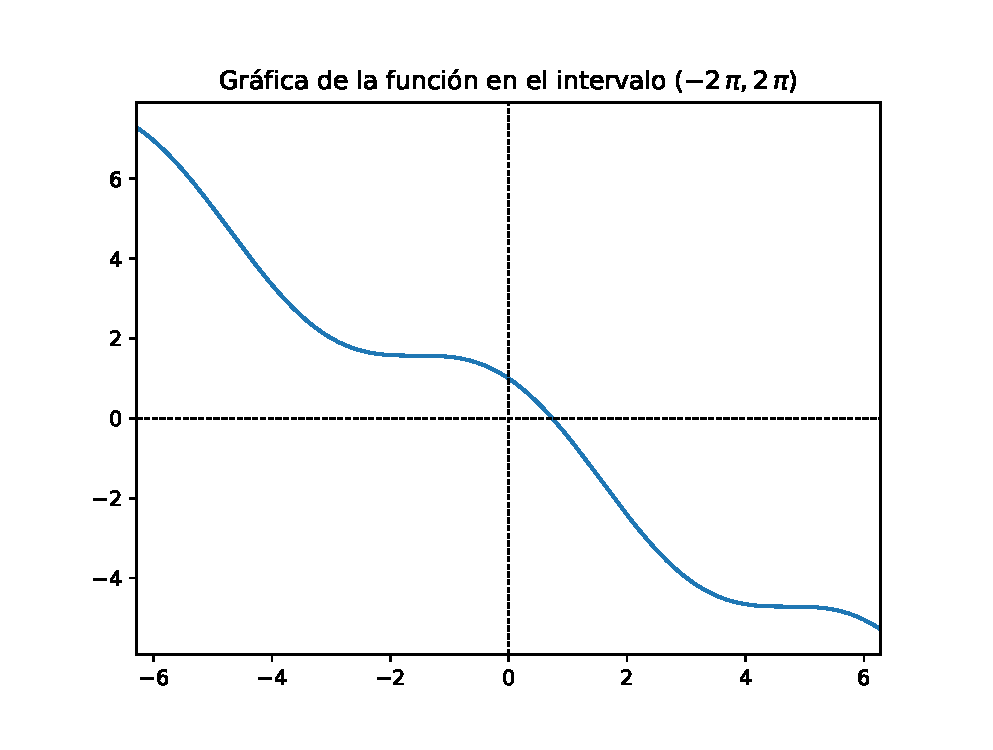
\includegraphics[scale=0.5]{Imagenes/raices_falsaposicion_01.eps}
	\caption{La gráfica nos ayuda de manera inicial para determinar el intervalo.}
\end{figure}
\end{frame}
\begin{frame}
\frametitle{Reducción del intervalo}
De manera general identificamos un intervalo, se recomienda usar el método de incrementos sucesivos.
\\
\bigskip
Recuerden que se deben de utilizar las herramientas que hemos desarrolla previamente.
\end{frame}
\begin{frame}
\frametitle{Reducción del intervalo}
\begin{figure}[h!]
	\centering
	\includegraphics[scale=0.5]{Imagenes/raices_falsaposicion_02.eps}
	\caption{Ya contamos con más información sobre el intervalo.}
\end{figure}
\end{frame}
\begin{frame}[allowframebreaks, fragile]
\frametitle{Código para el ejercicio}
\begin{lstlisting}[caption=Código para resolver el ejercicio, style=codigopython]
from ModuloRaices import FalsPos

def f(x):
	return np.cos(x) - x

a, b = 0., 1

raiz, bandera = FalsPos(f, a, b)

if bandera == 0:
	print('Se encontro la raiz en x = {0:1.10f}'.format(raiz))
elif bandera == 1:
	print('No hay raices en el intervalo ({0:1.3f}, {1:1.3f})'.format(a, b))
else:
	print('Se excedio el numero de iteraciones')
\end{lstlisting}
\end{frame}
\begin{frame}
\frametitle{Solución gráfica}
Incorporando una rutina de graficación, tendremos el siguiente resultado:
\begin{figure}[h!]
	\centering
	\includegraphics[scale=0.4]{Imagenes/raices_falsaposicion_03.eps}
	\caption{Gráfica con la raíz calculada con el método de la falsa posición.}
\end{figure}
\end{frame}
\begin{frame}
\frametitle{Ejercicio para resolver}
Con el método de la falsa posición calcula las raíces positivas de la función:
\begin{align*}
f(x) = \exp(x) - 3 \, x^{2}
\end{align*}
Utiliza todas las herramientas y técnicas de programación necesarias para obtener el resultado en una sola ejecución, es decir, si tiene dos o más raíces, se deben de mostrar en una sola corrida del programa.
\end{frame}
\begin{frame}
\frametitle{Resultado}
Deberás de obtener lo siguente:
\begin{figure}[h!]
	\centering
	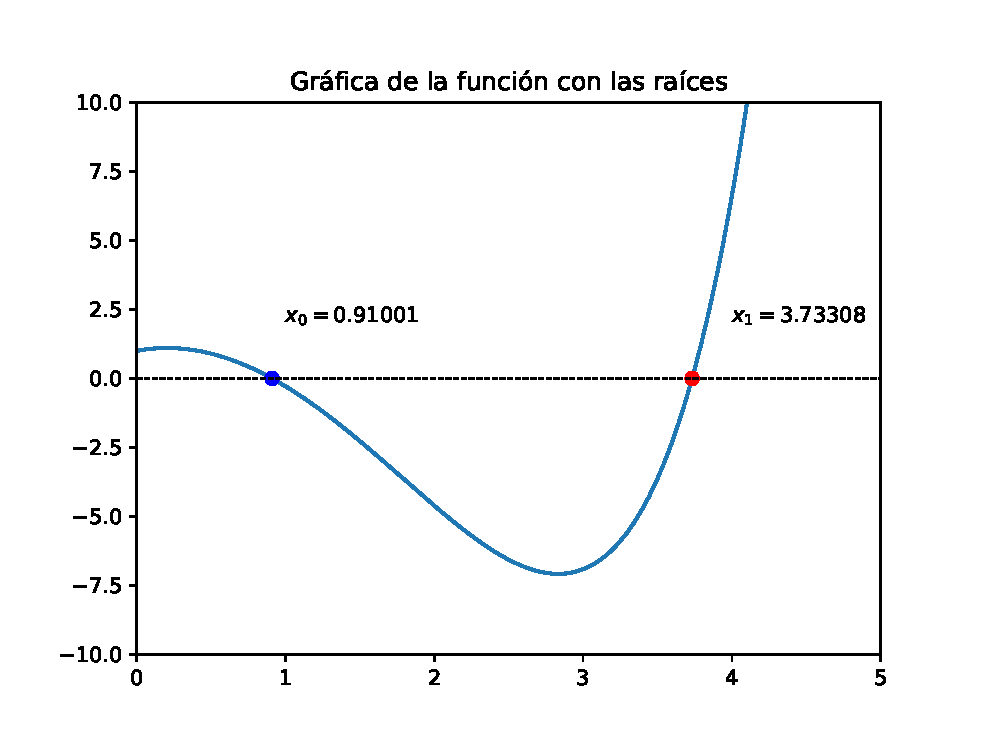
\includegraphics[scale=0.4]{Imagenes/raices_falsaposicion_04.eps}
	\caption{Deberás enviar el código más una gráfica como esta.}
\end{figure}
\end{frame}
\subsection{Método de la secante}
\begin{frame}
\frametitle{Método de la secante}
El método secante representa una compensación entre la eficiencia del método de Newton y los inconvenientes causados por la necesidad de una evaluación complementaria de la primera derivada de la función cuyos ceros son los que queremos encontrar.
\end{frame}
\begin{frame}
\frametitle{Método de la secante}
La mayor simplificación de este método es que la derivada ya no entra en las correcciones sucesivas, sin embargo, se obtiene de una relación de recurrencia que involucra tres (en lugar de dos) aproximaciones sucesivas de la raíz.
\end{frame}
\begin{frame}
\frametitle{Consideraciones del método}
Supondremos que la función $f(x)$ es casi lineal en la vecindad de la raíz y la recta determinada por los puntos $(x_{i-1}, f(x_{i-1}))$ y $(x_{i}, f(x_{i}))$, que corresponden a las dos aproximaciones, como se aprecia en la siguiente figura.
\end{frame}
\begin{frame}[fragile]
\frametitle{Método de la secante}
\begin{figure}[h!]
	\centering
	\includegraphics[scale=0.5]{Imagenes/raices_metodosecante_01.png}
	\caption{Secuencia de aproximaciones a la raíz.}
\end{figure}
% \setbeamercovered{invisible}
% \begin{center}
% 	\begin{tikzpicture}[font=\small]
% 		\draw [->] (0, 0) -- (7.5, 0);
% 		\draw [->] (0, 4) -- (0, -2);
% 		\draw [red, thick](7, 3.5) .. controls (6.5, 0.5) and (4.5, 0) .. (1, -1);
		

% 		\draw (1, 0.5) node {$a$};
% 		\draw [dashed] (1, 0) -- (1, -1);
% 		\draw (7, -0.5) node {$b$};
% 		\draw [dashed] (7, 0) -- (7, 3.6);
		
% 		\draw (6.2,-0.3) node {$x_{i-1}$};
% 		\draw (6, 1.6) node {$f_{i-1}$};
% 		\draw [dashed] (6.2, 0) -- (6.2, 1.33);

% 		\draw (5, -0.3) node {$x_{i}$};
% 		\draw (5, 1.8) node {$f_{i}$};
% 		\draw [dashed] (5, 0) -- (5, 1.3);
		
% 		\draw (6, 2) -- (4, 0);\pause

% 		\draw (4,-0.3) node {$x_{2}$};
% 		\draw [dashed] (4.1,0) -- (4.1,0.8);
% 		\draw (3.9, 1) node {$f_{2}$};\pause
% 		\draw (5.5,1.65) -- (2.9,0);
% 		\draw (2.8,-0.3) node {$x_{3}$};
% 	\end{tikzpicture}
% \end{center}
\end{frame}
\begin{frame}
\frametitle{Consideraciones del método}
La relación de recurrencia para el método secante se puede obtener simplemente aproximando la derivada en la fórmula de Newton-Raphson:
\begin{align*}
x_{i+1} = x_{i} - \dfrac{f(x_{i})}{f^{\prime}(x_{i})}
\end{align*}
\end{frame}
\begin{frame}
\frametitle{Consideraciones del método}
Por una expresión de diferencias finitas hacia atrás que involucra los tres aproximaciones:
\begin{align*}
f^{\prime}(x_{i}) \approx \dfrac{f(x_{i}) - f(x_{i-1})}{x_{i} - x_{i-1}}
\end{align*}
\end{frame}
\begin{frame}
\frametitle{Relación de recurrencia}
Entonces la relación de recuerrencia obtenida es la siguente:
\begin{align*}
x_{i+1} = x_{i} - f(x_{i}) \, \dfrac{x_{i} - x_{i-1}}{f(x_{i}) - f(x_{i-1})}
\end{align*}
\pause
que nos permite el cálculo de la aproximación $x_{i+1}$ de la raíz en base a las aproximaciones anteriores
$x_{i}$ y $x_{i-1}$.
\end{frame}
\begin{frame}
\frametitle{Tolerancia del método}
Este método iterativo se detiene hasta que la corrección de la raíz es menor a un valor de tolerancia predefino $\varepsilon$:
\begin{align*}
\abs{x_{i+1} - x_{i}} \leq \varepsilon \, \abs{x_{i+1}}
\end{align*}
\end{frame}
\begin{frame}
\frametitle{Valores iniciales}
Para iniciar la recurrencia, uno puede tomar, en principio, cualquier aproximación inicial arbitraria $x_{0}$ y $x_{1}$.
\\
\bigskip
Sin embargo, a partir de una única aproximación inicial $x_{0}$, se puede obtener la segunda aproximación aplicando un solo paso del método de aproximaciones sucesivas:
\begin{align*}
x_{1} = x_{0} - f(x_{0})
\end{align*}
\end{frame}
\begin{frame}
\frametitle{Comparación entre métodos}
La principal diferencia entre los métodos de la secante y de la falsa posición, es el hecho de que, si bien el método de la secante siempre emplea dos aproximaciones que, sin embargo, no necesariamente encierran la raíz.
\end{frame}
\begin{frame}
\frametitle{Comparación entre métodos}
El método de la falsa posición mantiene dos aproximaciones no necesariamente consecutivas que, sin embargo, corresponden a valores de función de signo opuesto, por lo tanto, incluyen implícitamente la raíz.
\end{frame}
\begin{frame}
\frametitle{Comparación entre métodos}
Aunque generalmente converge más rápido, al no delimitar necesariamente la raíz, el método de la secante no garantiza la convergencia para funciones insuficientemente suaves.
\end{frame}
\begin{frame}[allowframebreaks, fragile]
\frametitle{Código del método de la secante}
\begin{lstlisting}[caption=Código para el método de la secante, style=codigopython]
from math import fabs

def Secante(Func, a, b, x):
	eps = 1e-10
	itmax = 1000
	xA_0_B = x; fA_0_B = Func(xA_0_B)
	x = xA_0_B - fA_0_B

	for it in range(1, itmax+1):
		f = Func(x)
		df = (f - fA_0_B)/(x - xA_0_B)
		xA_0_B = x; fA_0_B = f
		dx = -f/df if fabs(df) > eps else - f
		x += dx

		if ((x < a) or (x > b)): return (x, 1)
		if (fabs(dx) <= eps*fabs(x)): return (x, 0)
	
	print("Se excedio el numero maximo de iteraciones!"); return (x, 2)
\end{lstlisting}
\end{frame}
\begin{frame}
\frametitle{Explicación del método}
Nuevamente se ha incluido una bandera para identificar la ejecución del código, revisa la tabla del método de la falsa posición, el significado de las banderas es el mismo.
\end{frame}
\begin{frame}
\frametitle{Explicación del método}
Se incrementó el número de iteraciones en \textoazul{itmax} (¿podría ser menor este valor?), el segundo valor de la aproximación inicial, se calcula con $x$.
\\
\bigskip
Dentro del ciclo \funcionazul{for} se realiza la aproximación de la derivada, se almacena la abscisa y el valor de la función, se realiza la corrección de la raíz con \funcionazul{dx}, y se continua avanzando en el intervalo.
\end{frame}
\begin{frame}[fragile]
\frametitle{Ejercicio}
Con el método de la secante, calcula la raíz de
\begin{align*}
f(x) = x - \sin x - 0.25 = 0
\end{align*}
Para la aproximación inicial $x_{0}$ elaboramos un gráfica para determinar ese valor.
\end{frame}
\begin{frame}
\frametitle{Gráfica de la función}
De la gráfica podemos elegir el valor $x_{0} = 1.$ y ocupar el código anterior.
\begin{figure}[h!]
	\centering
	\includegraphics[scale=0.4]{Imagenes/raices_secante_01.eps}
	\caption{Gráfica general de la función}
\end{figure}
\end{frame}
\begin{frame}[allowframebreaks, fragile]
\frametitle{Código}
\begin{lstlisting}[caption=Código para la solución con el método de la secante, style=codigopython]
from ModuloRaices import Secante
import numpy as np

def f(x):
    return x - np.sin(x) - 0.25

xA_0_B = 1.
a, b = 0., 2.

raiz, bandera = Secante(f, a, b, xA_0_B)
    
if bandera == 0:
    print('Se encontro la raiz en x = {0:1.10f}'.format(raiz))
elif bandera == 1:
    print('No hay raices en el intervalo ({0:1.3f}, {1:1.3f})'.format(a, b))
else:
	print('Se excedio el numero de iteraciones')
\end{lstlisting}
\end{frame}
\begin{frame}
\frametitle{Resultado}
\begin{figure}[h!]
	\centering
	\includegraphics[scale=0.5]{Imagenes/raices_secante_02.eps}
	\caption{Resultado del cálculo de la raíz.}
\end{figure}
\end{frame}
\begin{frame}
\frametitle{Ejercicio para resolver}
Con el método de la secante calcula las raíces de
\begin{align*}
x^{3} + 3 \, x^{2} - 1  = 0
\end{align*}
Justifica todo el procedimiento previo que debas de realizar para determinar $(a, b)$ y $x_{0}$.
\end{frame}
\end{document}